%% 
%% Copyright 2019-2024 Elsevier Ltd
%% 
%% Version 2.4
%% 
%% This file is part of the 'CAS Bundle'.
%% --------------------------------------
%% 
%% It may be distributed under the conditions of the LaTeX Project Public
%% License, either version 1.2 of this license or (at your option) any
%% later version.  The latest version of this license is in
%%    http://www.latex-project.org/lppl.txt
%% and version 1.2 or later is part of all distributions of LaTeX
%% version 1999/12/01 or later.
%% 
%% The list of all files belonging to the 'CAS Bundle' is
%% given in the file `manifest.txt'.
%% 
%% Template article for cas-dc documentclass for 
%% double column output.

%\documentclass[a4paper,fleqn,longmktitle]{cas-dc}
\documentclass[a4paper,fleqn]{cas-sc}

\usepackage{lmodern}
\usepackage[numbers]{natbib}
\usepackage{xcolor}
\usepackage{amsmath,amsfonts,amssymb,bm}
\usepackage{array}
\usepackage{textcomp}
\usepackage{graphicx}
\usepackage{booktabs}
\usepackage{pifont}
\usepackage{placeins}
\usepackage{duetalgorithm}

\setcounter{topnumber}{5}
\setcounter{bottomnumber}{2}
\setcounter{totalnumber}{7}
\renewcommand{\topfraction}{0.95}
\renewcommand{\bottomfraction}{0.85}
\renewcommand{\textfraction}{0.05}
\renewcommand{\floatpagefraction}{0.80}

\definecolor{draftred}{HTML}{B42318}
\definecolor{motionblue}{HTML}{1559B7}
\definecolor{appearanceorange}{HTML}{D95F02}
\definecolor{modulegreen}{HTML}{0F766E}

\newcommand{\gm}{g_t^{\mathrm{KF}}}
\newcommand{\ga}{g_t^{\mathrm{EMA}}}
\newcommand{\gbase}{\bm{g}_t^{0}}
\newcommand{\gfinal}{\bm{g}_t}

\begin{document}
\let\WriteBookmarks\relax
\def\floatpagepagefraction{1}
\def\textpagefraction{.001}

\shorttitle{Leveraging social media news}
\shortauthors{Shangqing Nie et~al.}

\title[mode=title]{SHUTrack: Learning to Suppress Harmful State Updates for Online Multi-Object Tracking}

\author[1,3]{Shangqing Nie}[orcid=0009-0003-8557-9313]
\ead{niesq25@mails.jlu.edu.cn}
\credit{Writing -- original draft, Visualization, Validation, Methodology, Formal analysis, Conceptualization}

\author[1,2,3]{Shengsheng Wang}[orcid=0000-0002-8503-8061]
\ead{wss@jlu.edu.cn}
\credit{Writing -- original draft, Validation}

\author[1,3]{Jiarui Zhao}[orcid=0009-0008-5266-5043]
\ead{zhaojr24@mails.jlu.edu.cn}
\credit{Validation, Formal analysis}

\author[2,3]{Yukuan Zhang}[orcid=0000-0002-2811-0936]
\cormark[1]
\ead{zyk24@mails.jlu.edu.cn}
\credit{Writing -- review and editing, Supervision, Conceptualization}

\address[1]{College of Software, Jilin University, Changchun 130012, China}
\address[2]{College of Computer Science and Technology, Jilin University, Changchun 130012, China}
\address[3]{Key Laboratory of Symbolic Computation and Knowledge Engineering of Ministry of Education, Jilin University, Changchun 130012, China}

\cortext[cor1]{Corresponding author}

\begin{abstract}
Online multi-object tracking relies on matched detections to continually update track states, but a detection that supports the current association may still cause a harmful update. An inaccurate bounding box or a corrupted appearance feature can enter the track state and affect later predictions and associations. The same detection may also have different effects on motion and appearance, making it difficult to decide which updates should be allowed. To address this problem, we propose SHUTrack, a framework that learns to suppress harmful state updates after association. Its main idea is to assess an update by its effect on the existing track state. During training, SHUTrack compares the later effects of updating the state with a matched detection and retaining the state before that update. This comparison provides a learning signal for deciding when an update should be reduced. A Harm-Aware Update Controller (HUC) makes separate update decisions for motion and appearance, while a Reliability-Guided Update Calibrator (RUC) refines these decisions using track context. Together, they limit harmful updates while allowing the tracker to adapt to target changes. Experiments on MOT17, MOT20, and SportsMOT show consistent improvements over TrackTrack in association accuracy and identity consistency. SHUTrack achieves HOTA scores of 67.8, 66.4, and 76.5 on the three benchmarks, respectively, with higher IDF1 and fewer identity switches on all three test sets.
\end{abstract}

\begin{keywords}
Online Multi-Object Tracking \sep State Assimilation \sep Counterfactual Supervision \sep Appearance Memory \sep Temporal Reliability
\end{keywords}

\maketitle

\section{Introduction}
Multi-object tracking (MOT) aims to localize multiple objects in video while preserving their identities over time. It supports applications including autonomous driving \cite{geiger2012we}, intelligent surveillance \cite{yin2019large}, sports analytics \cite{cui2023sportsmot}, and human behavior analysis \cite{kong2022human}. Tracking-by-detection (TBD) remains the dominant online formulation: a detector first produces frame-level observations, and the tracker links them into trajectories using motion, appearance, and geometric evidence \cite{bewley2016simple,wojke2017simple,zhang2022bytetrack,cao2023observation,aharon2022bot}. As object detectors have improved, the main difficulty has increasingly shifted from localizing an object in one frame to preserving a reliable state through occlusion, crowding, abrupt motion, and ambiguous appearance.

Most online trackers maintain at least two recursive forms of track memory. A Kalman state summarizes location, scale, velocity, and their uncertainty, while an appearance prototype aggregates ReID observations for later identity association. Once a detection is assigned to a track, the standard implementation updates both memories. The Kalman filter corrects its prediction with the detection box, and an exponential moving average (EMA) incorporates the detection embedding into the track prototype. This design is efficient and usually appropriate, but it embeds a strong assumption: if an association has been accepted, then the associated observation is sufficiently reliable to be written into every state.

Acceptance and reliability are not equivalent. Association chooses the best available assignment under the current candidate set and threshold; it does not guarantee that the selected box is accurately localized or that its feature is visually clean. In a crowded scene, the accepted box can be shifted toward a neighbor. Under partial occlusion, the ReID feature can contain foreground from another identity. During abrupt motion, an otherwise correct match can still be inconsistent with the short-term trajectory model. If such an observation is fully assimilated, the effect does not end at the current frame. A corrupted Kalman posterior biases the next prediction and changes later geometric costs, while a corrupted appearance prototype affects future ReID distances. The resulting error can therefore propagate even when the original association was technically correct.

\begin{figure}[pos=!ht]
    \centering
    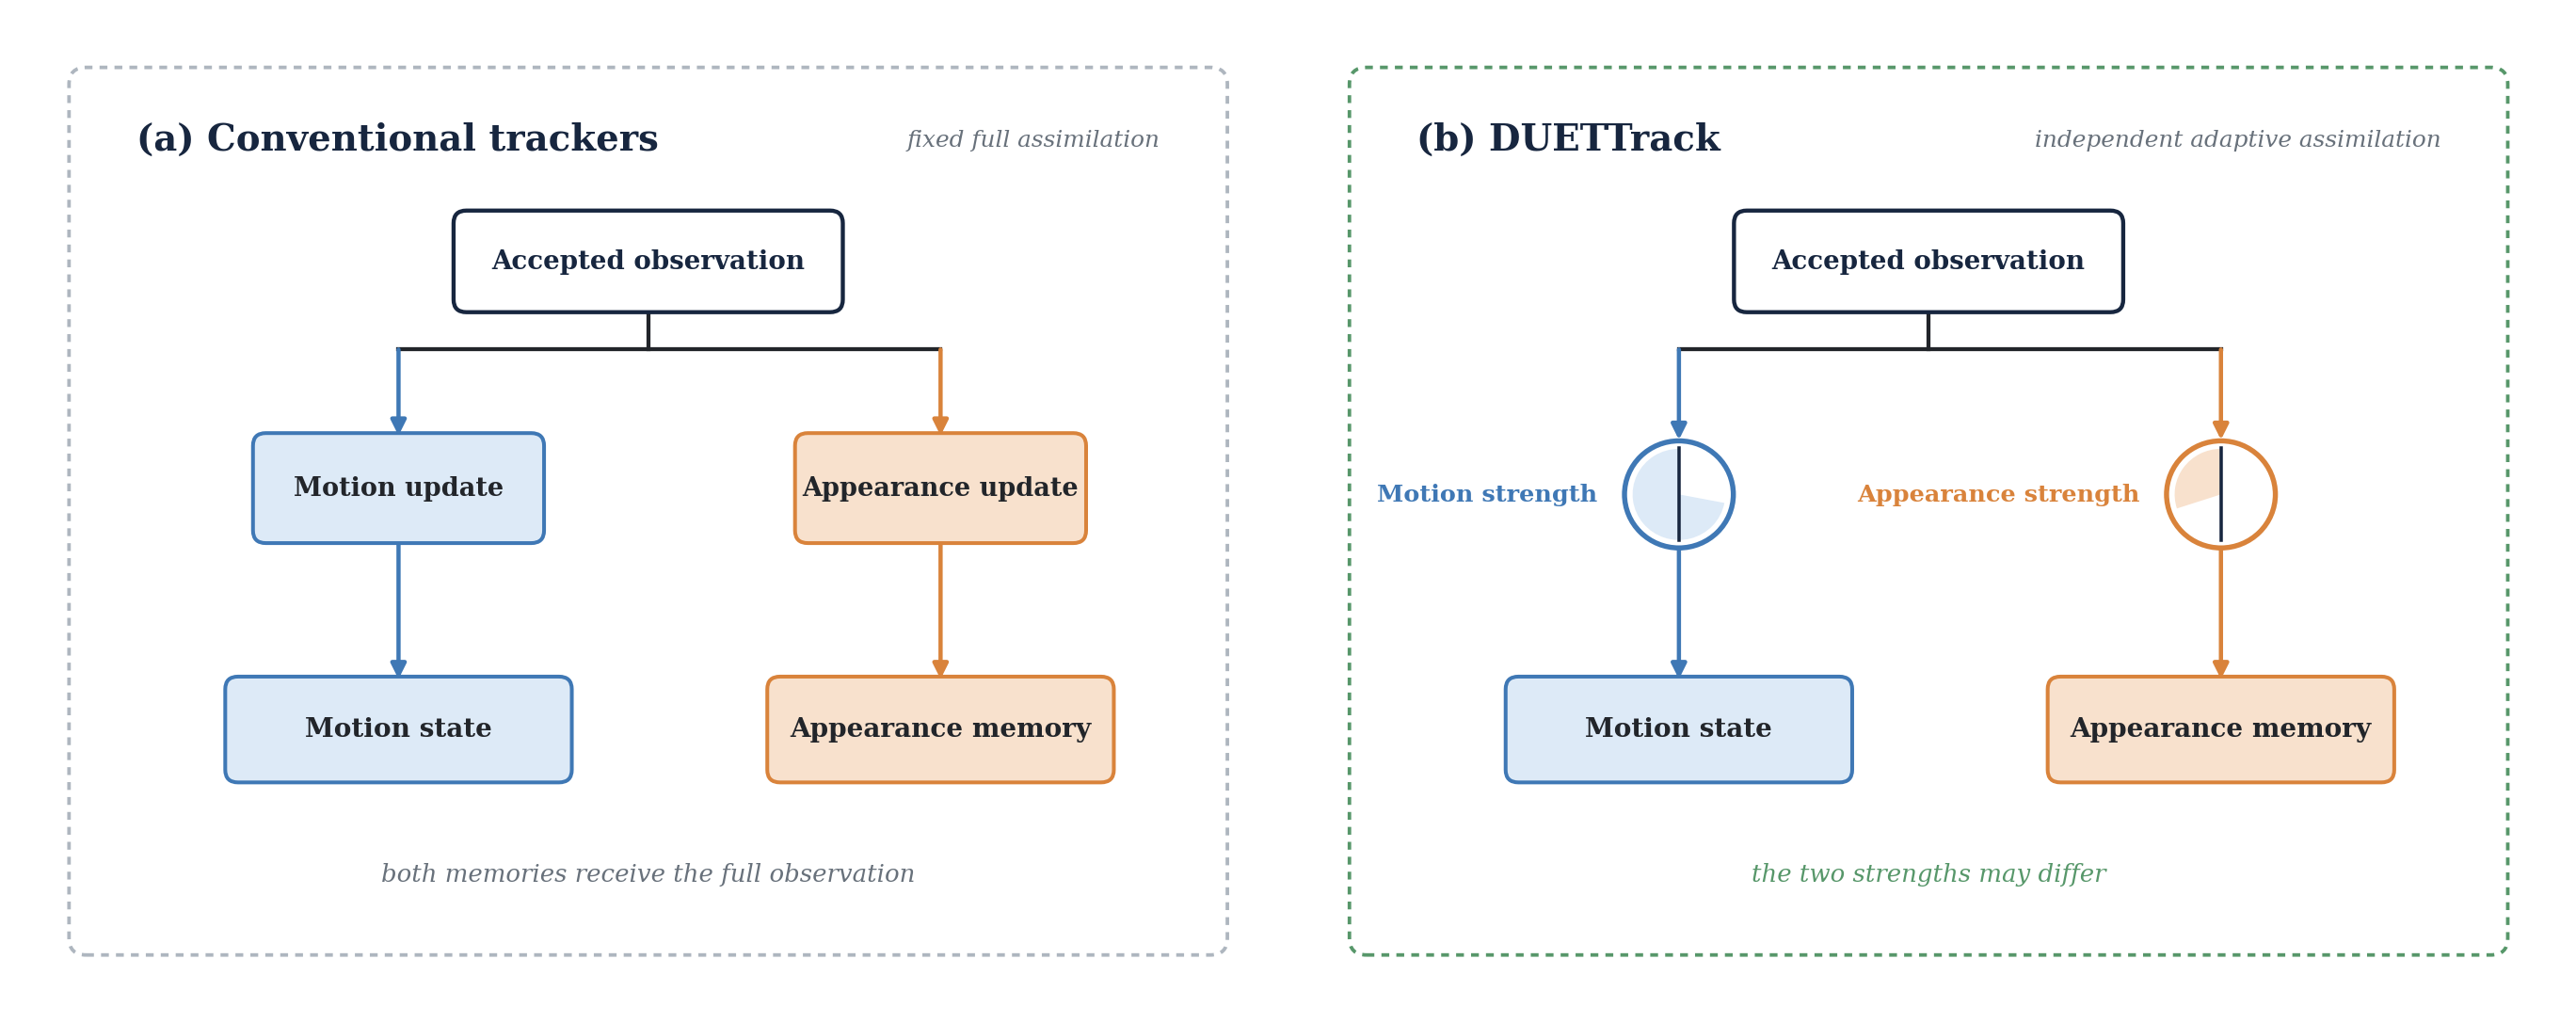
\includegraphics[width=\linewidth]{figures/fig1_motivation_v8.png}
    \caption{Conceptual comparison of post-association state assimilation. Conventional trackers apply an accepted observation directly to both the motion state and the appearance memory. DUETTrack instead estimates separate assimilation strengths for the two updates. The clock-like dials denote relative update strength rather than time or calibrated probability.}
    \label{fig:motivation}
\end{figure}

Fig.~\ref{fig:motivation} contrasts the two post-association update strategies. Conventional trackers perform full motion and appearance updates once a detection is accepted. DUETTrack preserves the accepted association but regulates how strongly that observation enters the motion state and appearance memory. The unequal dial settings illustrate that the two strengths need not agree: a well-localized but heavily occluded detection may be useful for motion correction and harmful to the appearance prototype, while a slightly displaced box may retain a clean identity feature but be unsuitable for geometric assimilation.

Existing trackers primarily improve what happens before or during association. ByteTrack \cite{zhang2022bytetrack} recovers low-confidence detections, OC-SORT \cite{cao2023observation} emphasizes observation-centric motion correction, StrongSORT \cite{du2023strongsort} and BoT-SORT \cite{aharon2022bot} enhance appearance and camera-motion handling, and TrackTrack \cite{shim2025focusing} reorganizes candidate utilization from the track perspective. Other approaches estimate detection uncertainty \cite{jung2024conftrack,solano2024utrack}, learn trajectory dynamics \cite{xiao2024motiontrack,lv2024diffmot,hu2026trackssm}, or maintain richer temporal memories \cite{cai2022memot,gao2023memotr}. These developments improve candidate generation, matching, or state prediction. Nevertheless, a focused question remains underexplored: after a match has already been accepted, how much future value does its box and appearance feature provide to the corresponding recursive state?

We address this question with DUETTrack, a utility-guided dual-state assimilation framework. Acting on accepted associations, DUETTrack estimates two continuous coefficients. The first controls interpolation between the Kalman prediction and its full measurement posterior; the second controls interpolation between the stored appearance prototype and its updated estimate. This formulation separates observation ownership from observation utility, allowing a tracker to retain a match while limiting its influence on future states.

The central challenge is supervision. A current detection can look plausible but still harm future tracking, and no direct annotation states whether its motion or appearance should be written. We therefore construct paired offline rollouts from the same pre-assimilation state. One branch fully writes the current observation and the other holds the existing state; both are propagated using the same future evidence. Their loss difference estimates the local future utility of the write action. Coverage and utility magnitude are used to turn this comparison into conservative soft targets, avoiding brittle binary decisions when the two branches are nearly equivalent or future evidence is incomplete.

DUETTrack contains two learned components. The Counterfactual Utility Estimator (CUE) models recent association, geometry, state, track-status, and appearance-interaction evidence. It combines interpretable policy estimation with a continuous offset to produce two base assimilation coefficients. The Cross-Evidence Calibrator (CEC) independently summarizes recent state--association and appearance-interaction histories, conditions their interaction on reliability evidence, and applies a bounded coefficient adjustment. This division assigns the primary decision to CUE while allowing CEC to make only a contextual local calibration.

Our contributions are summarized as follows.
\begin{itemize}
    \item We formulate post-association tracking as a dual-state assimilation problem in which an accepted detection can contribute differently to the Kalman state and the ReID prototype.
    \item We introduce paired write-versus-hold rollout supervision that estimates the local future utility of the current observation for the Kalman state and appearance prototype, and converts the estimates into confidence-aware soft targets without using future information online.
    \item We design CUE and CEC to combine interpretable policy estimation with reliability-aware cross-evidence calibration, yielding independent continuous controls for geometric and appearance-state assimilation.
    \item On the MOT17, MOT20, and SportsMOT test sets, DUETTrack consistently improves HOTA, AssA, and IDF1 over TrackTrack and reduces identity switches, with the largest fragmentation reduction observed on SportsMOT. A controlled MOT20 perturbation study further shows slower degradation under position and size noise.
\end{itemize}

\section{Related Work}
\subsection{Online Multi-Object Tracking}
Tracking-by-detection decomposes MOT into frame-level detection and temporal association, retaining a modular online pipeline that can inherit advances in either component \cite{ciaparrone2020deep}. SORT \cite{bewley2016simple} established a lightweight baseline with Kalman prediction and Hungarian assignment \cite{kuhn1955hungarian}; DeepSORT \cite{wojke2017simple} added appearance embeddings and a matching cascade; and ByteTrack \cite{zhang2022bytetrack} recovered useful low-confidence detections through a second association stage.

Recent trackers improve the assignment boundary through observation-centric motion \cite{cao2023observation,maggiolino2023deep}, camera compensation and appearance matching \cite{aharon2022bot}, stronger embeddings and post-processing \cite{du2023strongsort}, complementary weak cues \cite{yang2024hybrid}, pseudo-depth decomposition \cite{liu2025sparsetrack}, and fine-grained visual representations \cite{ren2023focus}. AIPT \cite{zhang2024aipt} and RccTrack \cite{zhang2025robust} further address confusing targets and camera motion. End-to-end query trackers such as TrackFormer \cite{meinhardt2022trackformer} and MOTR \cite{zeng2022motr} instead couple detection, association, and recurrent query revision.

TrackTrack \cite{shim2025focusing}, our host tracker, organizes candidate utilization from the track perspective and jointly considers high-confidence, low-confidence, and redundant detections. DUETTrack leaves this construction and the resulting assignment unchanged. It operates at the exposed post-association boundary of a modular tracker: association decides which detection belongs to a track, whereas DUETTrack decides how strongly the accepted observation should enter the recursive states used by later associations.

\subsection{Motion State Estimation}
The Kalman filter \cite{kalman1960new} remains a standard motion backbone for online MOT because it provides efficient recursive prediction and measurement correction. SORT-style systems propagate position, scale, velocity, and covariance before matching and apply a measurement update after assignment. Subsequent methods improve this state estimator through camera compensation \cite{aharon2022bot}, observation re-updating \cite{cao2023observation}, ground-plane projection \cite{yi2024ucmctrack}, or confidence-dependent measurement noise \cite{jung2024conftrack}.

Learned estimators can augment analytical filtering when the assumed dynamics are incomplete, as illustrated by KalmanNet \cite{revach2022kalmannet}. In MOT, recurrent, Transformer, state-space, and diffusion models have been used to improve trajectory prediction \cite{han2022mat,xiao2024motiontrack,xiao2024mambatrack,hu2026trackssm,lv2024diffmot,luo2024diffusiontrack}. These approaches primarily improve the prediction or uncertainty model. DUETTrack instead retains TrackTrack's full Kalman posterior and learns a bounded interpolation between that posterior and the preceding prediction, preserving both host endpoints exactly.

\subsection{Appearance Memory}
Online trackers must also preserve identity evidence across frames. DeepSORT stores a gallery of recent descriptors \cite{wojke2017simple}, whereas many efficient systems recursively average matched embeddings into a compact EMA prototype. StrongSORT and BoT-SORT improve the descriptor or its use in matching, and FineTrack \cite{ren2023focus} learns more discriminative local and global features under occlusion.

Other work makes memory itself more expressive. Multi-track pooling jointly updates appearance memories in the presence of similar targets \cite{kim2021discriminative}; UTM aggregates identity-aware information across detection, embedding, and tracking components \cite{you2023utm}; and MeMOT and MeMOTR retain object information through learned temporal memories \cite{cai2022memot,gao2023memotr}. Polycepta \cite{nagy2026polycepta} further treats appearance as a recursive object-centric state. These methods motivate richer identity representations, but a matched feature can still be occluded or mixed with a neighbor. DUETTrack therefore controls whether the host EMA candidate should be stored, rather than replacing the ReID encoder or memory representation.

\subsection{Reliability-Aware Tracking}
Motion and appearance reliability are commonly used to improve the current association. Neural Gating \cite{kim2018neuralgating} learns to combine the two cues, ConfTrack \cite{jung2024conftrack} adapts filtering to detection confidence, and UTrack \cite{solano2024utrack} models uncertain detections during matching. U2MOT \cite{liu2023uncertainty} uses association uncertainty to rectify risky pseudo-tracklets, while path-consistency supervision enforces stable associations under different temporal observation paths \cite{lu2024self}. Together, these studies show that cue reliability is contextual rather than a fixed hand-crafted weight.

Reliability for matching is nevertheless different from utility for recursive storage. A high-confidence box can be displaced during overlap, and a correctly localized detection can yield a contaminated ReID crop. Conversely, an uncertain observation can be useful when it corrects a drifting prediction. DUETTrack therefore uses confidence and ambiguity as evidence, not as write targets, and predicts distinct Kalman-state and appearance-prototype coefficients. Its Cross-Evidence Calibrator further compares the recent state--association and appearance-interaction histories, but it only adjusts the already selected post-association action.

\subsection{Counterfactual Supervision}
Counterfactual learning evaluates how an outcome would change under an alternative action. In sequential decision problems, counterfactually guided policy search uses a structural model to compare alternative actions on logged trajectories \cite{buesing2018woulda}. Learning using privileged information similarly formalizes training with signals that are unavailable at deployment \cite{vapnik2009new}. Both ideas are relevant to our use of future evidence, but DUETTrack adopts a narrower supervised construction rather than a general causal or reinforcement-learning formulation.

For every training event, we branch from the same pre-assimilation state, apply one of two fixed actions---write or hold---and propagate both branches with identical future evidence. Their loss difference supplies a local utility target for the current state write. We do not infer unobserved outcomes from observational data, optimize an online policy, or rerun global assignment under each action. Future annotations are used only to construct offline targets; at test time, CUE and CEC receive a causal six-event history. This controlled scope prevents future information from entering online inference and avoids claiming a globally optimal counterfactual tracker.

\section{Methodology}
Let track $i$ at frame $t$ have a predicted Kalman state $(\bm{\mu}_{t}^{-},\bm{P}_{t}^{-})$ and a stored appearance prototype $\bm{f}_{t}^{-}$. TrackTrack assigns a detection $d_t=(\bm{z}_t,\bm{q}_t,s_t)$, where $\bm{z}_t$ is the box measurement, $\bm{q}_t$ is its ReID feature, and $s_t$ is its confidence. DUETTrack estimates $\gfinal=[\gm,\ga]\in[0,1]^2$ after this assignment. The two coefficients regulate how much of the full Kalman-state and EMA-prototype updates is assimilated.

\subsection{Framework Overview}
Fig.~\ref{fig:framework} places DUETTrack inside the unchanged TrackTrack pipeline. Detection, ReID extraction, candidate construction, cost computation, assignment, and track management are inherited from TrackTrack. We define a mature track as one in the tracked or lost state whose host history contains at least six entries. For each mature track, the accepted match and the track's preceding events form a left-padded causal window of length six. Matched events contain both track and detection information; unmatched events contain the track-side state and an explicit no-detection pattern. Reset masks prevent a window from crossing a terminated or reinitialized trajectory.

\begin{figure}[pos=!ht]
    \centering
    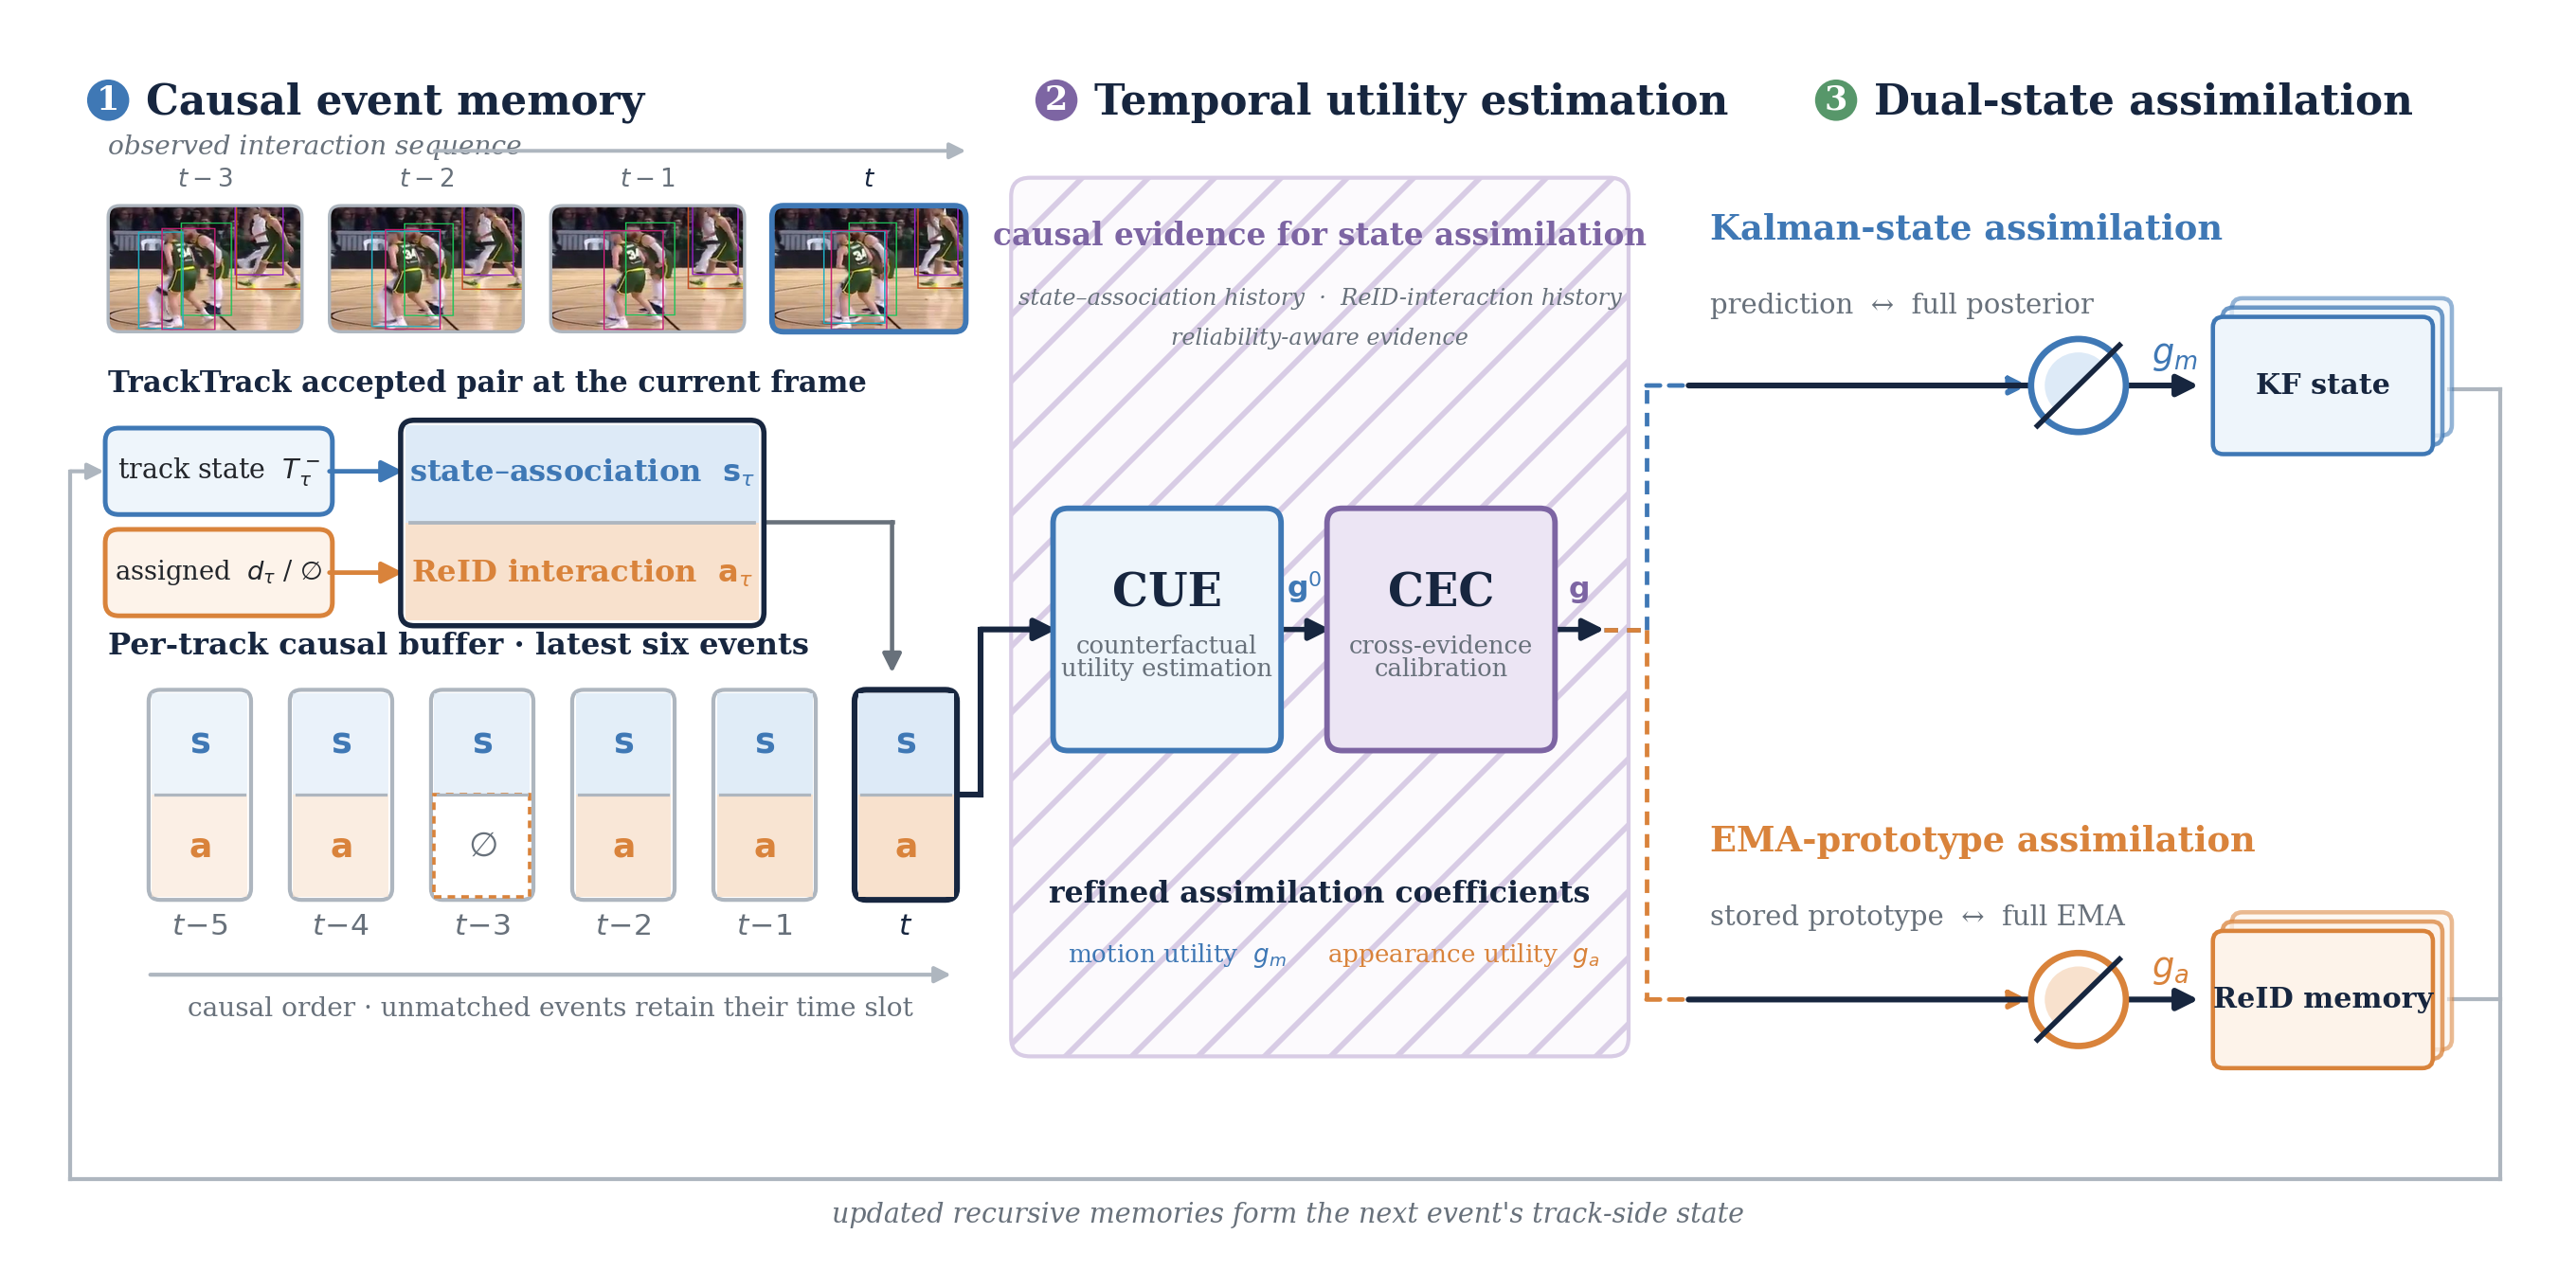
\includegraphics[width=\linewidth]{figures/fig2_framework_v12_cec.png}
    \caption{Framework overview of DUETTrack. An accepted TrackTrack pair is recorded as state--association and ReID-interaction evidence in a six-event causal memory. CUE produces the primary motion and appearance assimilation coefficients, CEC refines them using reliability-aware cross-evidence, and the resulting coefficients independently control the Kalman-state and EMA-prototype updates. Figs.~\ref{fig:cue} and \ref{fig:cec} detail the two learned components.}
    \label{fig:framework}
\end{figure}

The event is recorded before assimilation, so its track-side fields describe the state that produced the association rather than the consequence of the current decision. Per-track buffers are left-padded and use validity and reset masks. An unmatched event occupies a temporal position, allowing a later match to reveal a return after a gap.

For motion, we first compute the full Kalman measurement posterior using the original update rule,
\begin{equation}
(\bm{\mu}_{t}^{+},\bm{P}_{t}^{+})
=
\operatorname{KFUpdate}(\bm{\mu}_{t}^{-},\bm{P}_{t}^{-},\bm{z}_t,s_t).
\label{eq:full_kf}
\end{equation}
Instead of committing to this posterior, DUETTrack interpolates from the prediction:
\begin{align}
\bm{\mu}_{t}
&=
\bm{\mu}_{t}^{-}
+
\gm(\bm{\mu}_{t}^{+}-\bm{\mu}_{t}^{-}), \\
\bm{P}_{t}
&=
(1-\gm)\bm{P}_{t}^{-}
+
\gm\bm{P}_{t}^{+}.
\label{eq:motion_assimilation}
\end{align}
The covariance is symmetrized after interpolation. The effective history box is analogously formed between the predicted box and the accepted detection box. Therefore, $\gm=0$ exactly preserves the prediction, $\gm=1$ recovers the original full update, and intermediate values provide continuous correction.

Because $\bm{P}_{t}^{-}$ and $\bm{P}_{t}^{+}$ are positive semidefinite, their convex combination remains valid; symmetrization removes numerical asymmetry. The endpoint at $\gm=1$ is exactly the unmodified TrackTrack update, so the learned action is a deviation from the host rather than a replacement motion model.

For appearance, TrackTrack's confidence-aware EMA first produces the full candidate prototype
\begin{align}
\beta_t &= \alpha +(1-\alpha)(1-s_t), \\
\bm{f}_{t}^{+}
&=
\operatorname{norm}\!\left(
\beta_t\bm{f}_{t}^{-}+(1-\beta_t)\bm{q}_t
\right),
\label{eq:full_ema}
\end{align}
where $\alpha$ denotes the host appearance decay. DUETTrack then applies
\begin{equation}
\bm{f}_{t}
=
\operatorname{norm}\!\left(
(1-\ga)\bm{f}_{t}^{-}+\ga\bm{f}_{t}^{+}
\right).
\label{eq:appearance_assimilation}
\end{equation}
The endpoints again have exact semantics: $\ga=0$ retains the old prototype and $\ga=1$ reproduces the host EMA. The Kalman-state and EMA-prototype coefficients are not tied because localization and visual quality can diverge for the same detection.

The second interpolation targets TrackTrack's complete score-aware EMA candidate rather than the raw detection feature. It thus preserves the host confidence rule inside $\bm{f}_{t}^{+}$, while $\ga$ determines whether that candidate should enter long-term memory.

DUETTrack is applied only to accepted pairs of mature tracks. If the current event is unmatched, both coefficients and both CEC adjustments are set to zero; the unmatched event is nevertheless appended to the causal buffer so that missed observations and temporal gaps remain visible to future decisions. Newly initialized tracks follow TrackTrack's original initialization because they lack sufficient history for utility estimation.

The action space contains no reject or reassignment operation. DUETTrack cannot repair an already incorrect current-frame ID, but it can limit how a noisy observation propagates afterward. This restriction also prevents it from silently changing detection recall or association thresholds.

\subsection{Counterfactual Utility Estimator}
CUE combines an offline target-construction procedure with a causal estimator used at test time. No benchmark annotation directly specifies the desired values of $\gm$ and $\ga$. We therefore construct training targets by comparing two controlled actions from the same pre-assimilation state: \emph{write}, which applies the current full update, and \emph{hold}, which skips it. The remainder of each rollout is shared. This paired construction attributes the loss difference to the current action while avoiding a comparison between unrelated trajectories.

Formally, for modality $r\in\{m,a\}$, the branches start from identical $S_{t,r}^{-}$ and differ only through $S_{t,r}^{W}=\operatorname{Write}(S_{t,r}^{-},d_t)$ and $S_{t,r}^{H}=S_{t,r}^{-}$. Subsequent prediction, camera compensation, observations, and update rules are shared. This estimates a local intervention effect; global assignment is not rerun, because doing so would entangle the action with other trajectories and track-management outcomes.

\begin{figure}[pos=!ht]
    \centering
    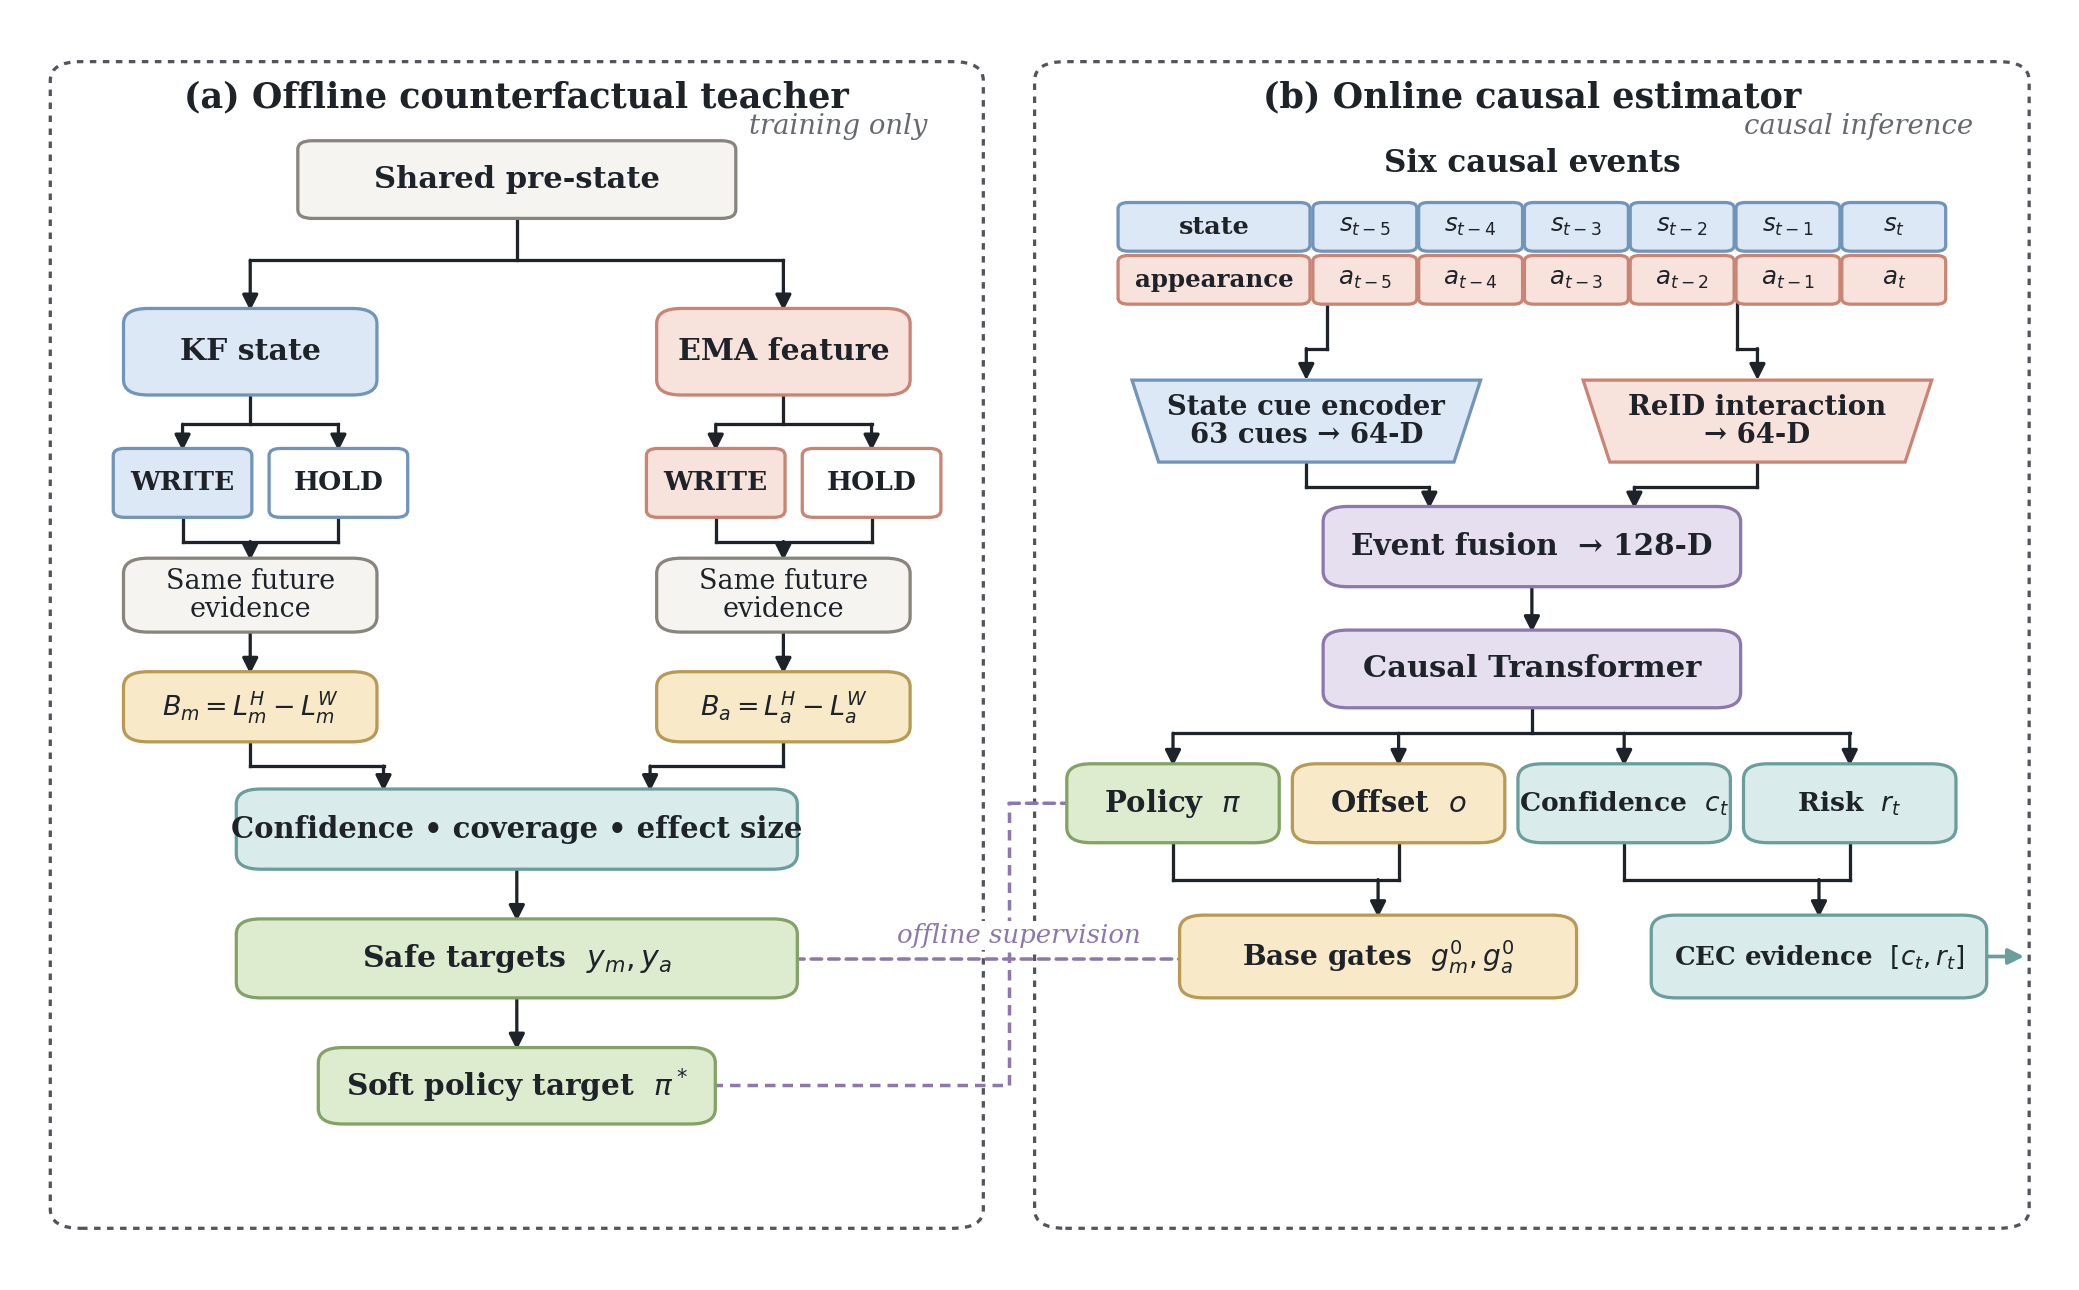
\includegraphics[width=\linewidth]{figures/fig3_cue_v12_offset.png}
    \caption{Counterfactual Utility Estimator. (a) The offline teacher compares write and hold from a shared pre-state under identical future evidence, then derives safe assimilation targets and soft policy supervision. (b) The online estimator separately encodes six causal state--association and ReID-interaction events before temporal modeling. Policy and offset outputs form the two base coefficients, while confidence and risk outputs provide explicit evidence to CEC.}
    \label{fig:cue}
\end{figure}

\paragraph{Kalman-state utility.}
For a matched training event, the write branch applies Eq.~\eqref{eq:full_kf}; the hold branch retains $(\bm{\mu}_{t}^{-},\bm{P}_{t}^{-})$. At the current frame and up to $K$ future frames, the predicted box $\hat{\bm{b}}_{\tau}$ is compared with the target ground-truth box $\bm{b}_{\tau}^{\mathrm{gt}}$ using
\begin{equation}
\ell_m(\tau)
=
1-\operatorname{IoU}(\hat{\bm{b}}_{\tau},\bm{b}_{\tau}^{\mathrm{gt}})
+
\lambda_{\mathrm{loc}}\ell_{\mathrm{L1,norm}}
(\hat{\bm{b}}_{\tau},\bm{b}_{\tau}^{\mathrm{gt}}).
\label{eq:motion_loss}
\end{equation}
The normalized $\ell_1$ term divides horizontal and vertical coordinate errors by the ground-truth width and height, and $\lambda_{\mathrm{loc}}$ balances it against the overlap term. At each future step, both branches receive the same camera warp, Kalman prediction, and optional detector observation. The future observation is the detector candidate with the highest IoU above $\theta_{\mathrm{match}}$ to the target ground truth; ground-truth boxes are used for loss only and are never inserted as Kalman measurements. Summing valid frames yields $L_m^{W}$ and $L_m^{H}$.

IoU captures overlap and scale, whereas normalized $\ell_1$ remains informative after overlap vanishes and avoids favoring large objects. A short horizon keeps the current action as the dominant difference between branches.

\paragraph{Appearance utility.}
The write branch applies the full EMA in Eq.~\eqref{eq:full_ema}, whereas the hold branch retains $\bm{f}_{t}^{-}$. Both then receive the same future target-aligned detector features through the original EMA. An offline identity prototype $\bm{p}_i$ is constructed from at least $N_{\mathrm{proto}}$ high-quality detections for identity $i$, each with IoU at least $\theta_{\mathrm{proto}}^{\mathrm{IoU}}$ and score at least $\theta_{\mathrm{proto}}^{\mathrm{score}}$. Appearance loss is
\begin{equation}
\ell_a(\tau)=1-\cos(\bm{f}_{\tau},\bm{p}_i),
\label{eq:appearance_loss}
\end{equation}
which produces $L_a^{W}$ and $L_a^{H}$ over valid frames. Target identity is resolved from observations preceding the current event; the current detection is not used to decide which identity the track represents.

The prototype requirement excludes identities with insufficient clean evidence and separates the reference from the feature under evaluation. Including the current detection in $\bm{p}_i$ would artificially favor the write branch through shared noise; the stated thresholds are label safeguards, not test-time filters.

For state type $r\in\{m,a\}$, the write benefit is
\begin{equation}
B_r=L_r^{H}-L_r^{W}.
\label{eq:benefit}
\end{equation}
A positive benefit means that writing the current observation reduces future loss, while a negative value favors holding the prior state. We first map the benefit to an oracle soft decision
\begin{equation}
y_r^{\mathrm{oracle}}
=
\sigma\!\left(\frac{B_r}{\tau_r}\right),
\qquad
\tau_r=
\operatorname{clip}\!\left(
\operatorname{median}_{B_r\neq0}|B_r|,
\tau_{\min},\tau_{\max}
\right).
\label{eq:oracle_soft}
\end{equation}
The confidence of this label combines evidence coverage $\rho_r$ with effect magnitude:
\begin{equation}
c_r
=
\rho_r
\min\!\left(\frac{|B_r|}{\kappa\tau_r},1\right).
\label{eq:label_confidence}
\end{equation}
Let $n_m$ denote the number of available target ground-truth boxes over the current frame and the $K$ future frames, and let $n_a$ denote the number of those future frames for which a detector box overlaps the target by more than $\theta_{\mathrm{match}}$. We use $\rho_m=n_m/(K+1)$ and $\rho_a=n_a/K$. The safe target is
\begin{equation}
y_r=c_r y_r^{\mathrm{oracle}}+(1-c_r).
\label{eq:safe_target}
\end{equation}
Thus, weak or incomplete counterfactual evidence falls back toward the host's full update rather than incorrectly suppressing a valid association. Finally, the dual target $\bm{y}=[y_m,y_a]$ is converted into a soft distribution over the five policy prototypes $\bm{p}_k$ using
\begin{equation}
\pi_k^{*}
=
\frac{\exp(-\|\bm{p}_k-\bm{y}\|_2^2/\tau_{\mathrm{policy}})}
{\sum_j\exp(-\|\bm{p}_j-\bm{y}\|_2^2/\tau_{\mathrm{policy}})}.
\label{eq:policy_target}
\end{equation}
All rollout construction is restricted to training data. Online tracking receives only causal event history and never accesses ground truth, target-aligned future detections, or identity prototypes.

The fallback is intentionally asymmetric: suppressing an observation on weak evidence may prevent recovery, whereas a target near one reproduces the established host. Strong holding therefore requires confident negative benefit. The soft policy target preserves uncertainty by distributing mass among nearby prototypes.

\paragraph{Causal estimator.}
CUE converts a causal sequence of track events into a primary dual-state decision, as summarized in Fig.~\ref{fig:cue}(b). Each event has a ReID-interaction branch and a structured state--association branch. The ReID-interaction branch projects the stored track feature and the current detection feature to 64 dimensions using a shared linear layer and LayerNorm. It concatenates the projected track feature, detection feature, their absolute difference, and element-wise product. A $256\!\rightarrow\!128\!\rightarrow\!64$ MLP produces a 64-dimensional appearance interaction token.

The structured state--association branch contains 63 cues in a fixed index order. Indices 0--26 contain seven pairwise scores (IoU similarity and distance, cosine, confidence, angle, raw cost, and final cost), the assignment threshold and normalized round, detection score, a three-way source one-hot, six row-cost and six column-cost statistics, maximum detection overlap, and a detection-presence indicator. Indices 27--54 contain four box residuals, normalized predicted and detected boxes, four size-normalized Kalman velocities, four image-normalized log covariance diagonals, and eight tracker-velocity components. Indices 55--62 contain the current, latest, and three-observation mean scores, clipped normalized history length and observation gap, and a new/tracked/lost one-hot. Each dimension is standardized by its training-set mean and standard deviation, with values below $10^{-8}$ replaced by one. For unmatched events, detection-dependent entries are zero while track-side cues remain available. A LayerNorm and a $63\!\rightarrow\!128\!\rightarrow\!64$ MLP produce the structured context token.

Cost margins and entropy describe assignment ambiguity; geometry and covariance describe motion agreement; track status and observation gap distinguish routine noise from reappearance. The appearance interaction retains both projected endpoints and symmetric comparisons, avoiding dependence on a single cosine distance.

The two tokens are concatenated and fused into a 128-dimensional event embedding $\bm{e}_t$. CUE retains the latest six embeddings, adds learned relative position embeddings, and processes them with a two-layer Transformer encoder with four attention heads and feed-forward dimension 256 \cite{vaswani2017attention}. Left padding is masked, and the representation at the current position summarizes the causal window.

Only the current position is decoded, so the estimator remains causal. The fixed six-event window captures short trends with bounded storage and includes unmatched events so that a returning track is not treated as temporally adjacent to its last clean match.

Instead of directly regressing two unrelated coefficients, CUE predicts a distribution $\bm{\pi}_t$ over five semantically interpretable policies:
\begin{equation}
\mathcal{P}
=
\{(1,1),(1,0),(0,1),(0,0),(0.5,0.5)\},
\label{eq:policy_set}
\end{equation}
corresponding to full write, Kalman-state only, EMA-prototype only, hold both, and soft caution. It also predicts a two-dimensional unconstrained offset $\bm{o}_t$. The base decision is
\begin{equation}
\gbase
=
\operatorname{clip}_{[0,1]}
\left(
\sum_{k=1}^{5}\pi_{t,k}\bm{p}_k
+
\delta_{\mathrm{CUE}}\tanh(\bm{o}_t)
\right).
\label{eq:cue_gate}
\end{equation}
The policy mixture supplies a structured prior over common dual-state actions, while the bounded offset represents continuous cases between them. This design keeps the output interpretable without forcing hard policy selection.

The prototypes do not discretize the final action: their mixture spans asymmetric cases, and the offset covers intermediate targets. The probabilities also expose whether uncertainty concerns overall caution or disagreement between evidence streams. The ablation study includes direct two-coefficient regression to isolate the value of this structured output.

Two detached auxiliary heads predict a three-dimensional utility-confidence cue $[c_m,c_a,\max(c_m,c_a)]$ and a four-dimensional risk cue $[1-y_m^{\mathrm{oracle}},1-y_a^{\mathrm{oracle}},1-\min(c_m,c_a),|y_m^{\mathrm{oracle}}-y_a^{\mathrm{oracle}}|]$. Detachment prevents these auxiliary objectives from changing the event representation learned by the primary base decision. Their outputs are instead used as explicit reliability evidence by CEC. At an unmatched current event, CUE is overridden by a deterministic hold-both sentinel with zero coefficients.

\subsection{Cross-Evidence Calibrator}
CUE makes the primary decision from fused event embeddings, but two events with similar current evidence may require different adjustments depending on how structured state--association evidence and ReID interaction evolved in the recent window. CEC therefore revisits the base coefficients using separated histories while remaining subordinate to CUE. We use \emph{cross-evidence} rather than cross-modal because the two streams are learned views of one tracking event, not distinct sensing modalities.

\begin{figure}[pos=!ht]
    \centering
    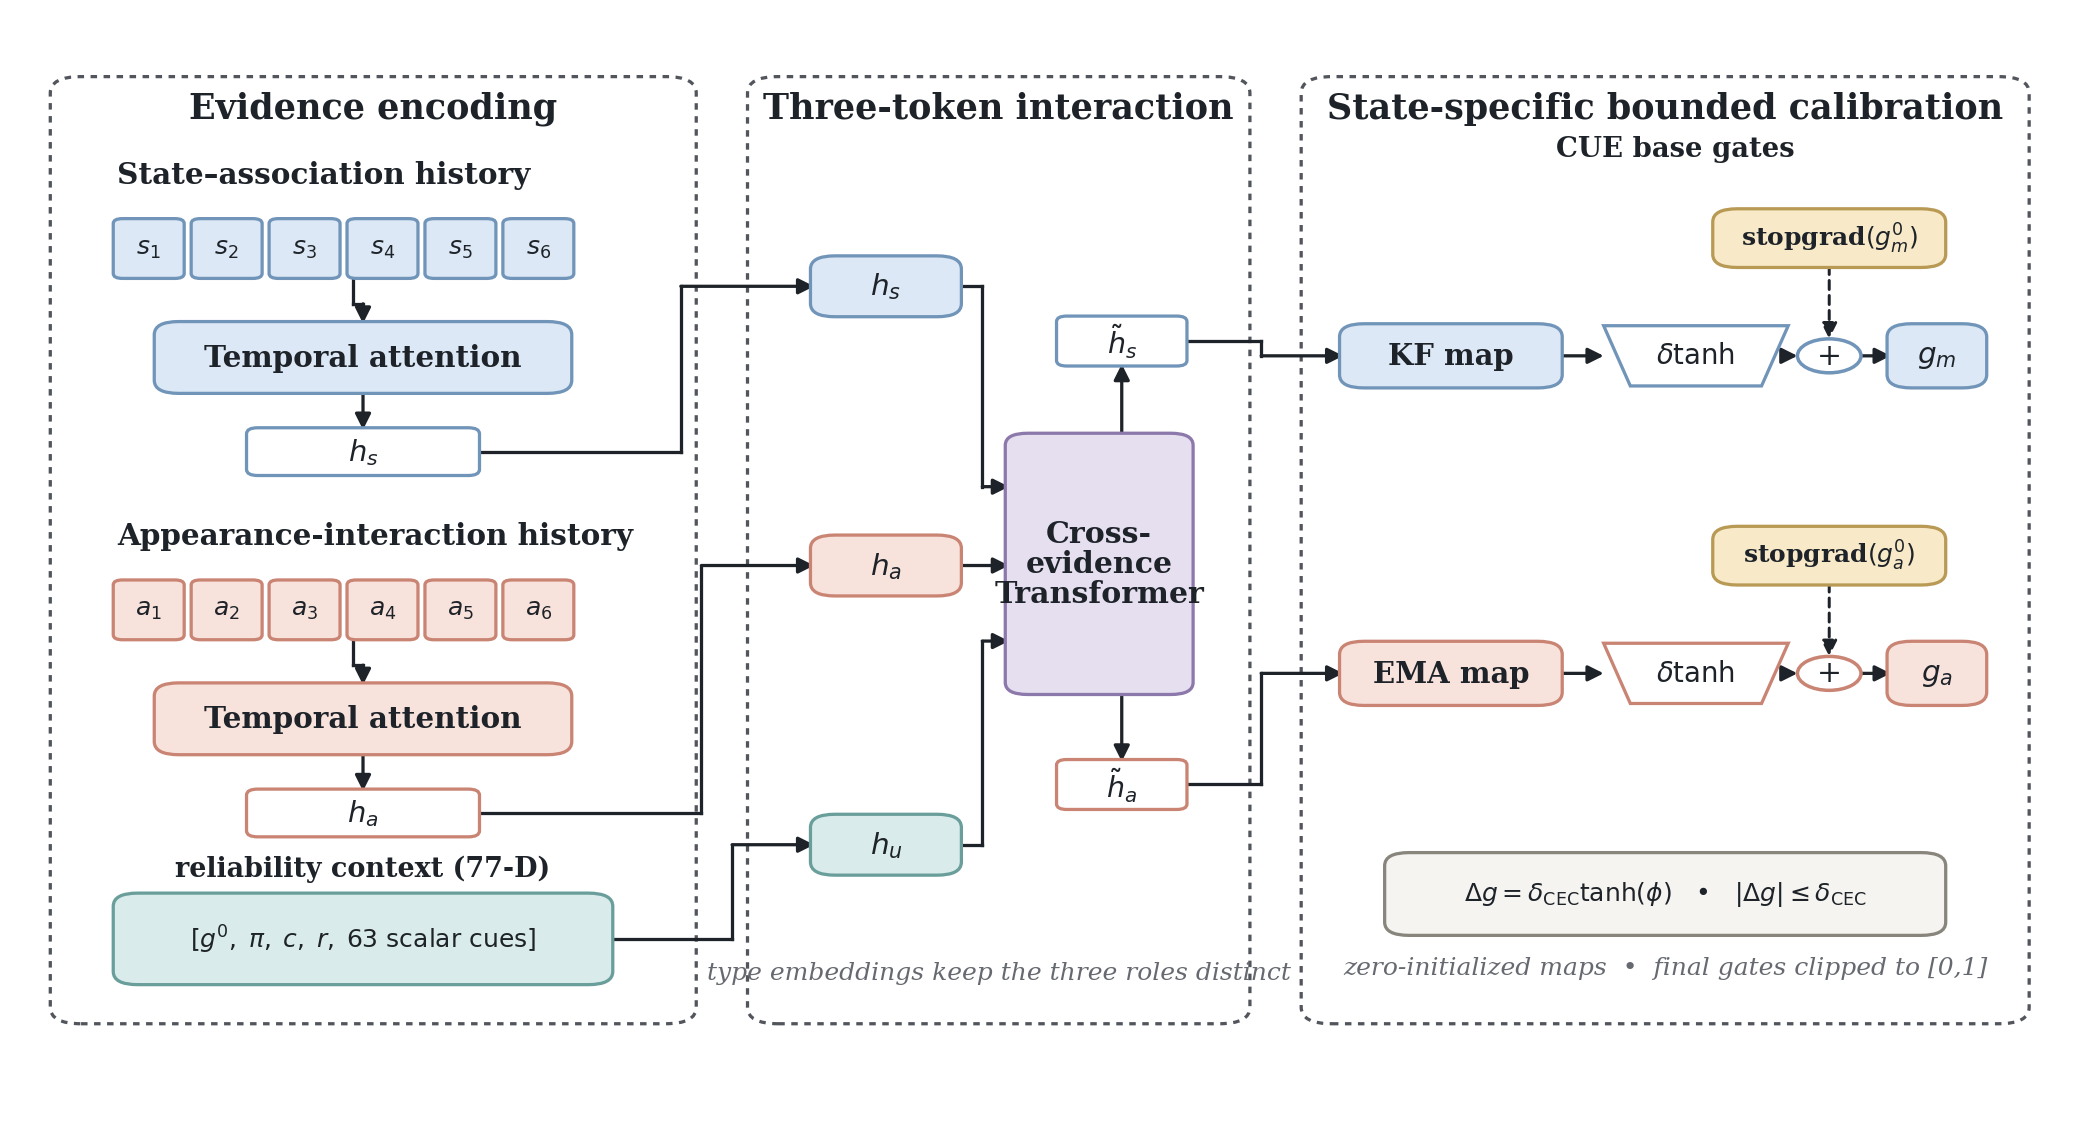
\includegraphics[width=\linewidth]{figures/fig4_cec_v12_imagegen.png}
    \caption{Cross-Evidence Calibrator. State--association and ReID-interaction histories are summarized independently and combined with an explicit reliability context through a three-token interaction. Two state-specific maps then refine the motion/Kalman and appearance/EMA coefficients. Stop-gradient paths preserve CUE as the primary estimator, while the calibrated coefficients remain local adjustments to its base decision.}
    \label{fig:cec}
\end{figure}

As illustrated in Fig.~\ref{fig:cec}, CEC receives the six 64-dimensional structured context tokens as state--association history and the six 64-dimensional interaction tokens as appearance history. Each stream is projected to 128 dimensions and augmented with an evidence-type embedding and a learned relative position embedding. Separate four-head temporal-attention modules use the current token as the query and the causal window as keys and values, producing summaries $\bm{h}_t^s$ and $\bm{h}_t^a$.

An explicit reliability vector concatenates the two base coefficients, five policy probabilities, three auxiliary cue values, four risk values, and the current 63 scalar features:
\begin{equation}
\bm{u}_t=
\left[
\gbase,\bm{\pi}_t,\bm{c}_t,\bm{r}_t^{\mathrm{risk}},\bm{s}_t
\right]\in\mathbb{R}^{77}.
\label{eq:reliability_vector}
\end{equation}
A linear projection produces a 128-dimensional reliability token $\bm{h}_t^u$. The three tokens $[\bm{h}_t^s,\bm{h}_t^a,\bm{h}_t^u]$ receive evidence-type embeddings and pass through a one-layer, four-head Transformer with feed-forward dimension 256. Separate calibration maps read the contextualized state--association and appearance positions and produce
\begin{equation}
\Delta\bm{g}_t
=
\delta_{\mathrm{CEC}}\tanh
\left(
\left[
\phi_{\mathrm{KF}}(\tilde{\bm{h}}_t^s),
\phi_{\mathrm{EMA}}(\tilde{\bm{h}}_t^a)
\right]
\right).
\label{eq:cec_delta}
\end{equation}
The final decision is
\begin{equation}
\gfinal
=
\operatorname{clip}_{[0,1]}
\left(\operatorname{stopgrad}(\gbase)+\Delta\bm{g}_t\right).
\label{eq:final_gate}
\end{equation}
Zero initialization of the final calibration maps makes CEC start as the identity mapping. The $\pm\delta_{\mathrm{CEC}}$ range prevents the calibrator from replacing the CUE decision and establishes a clear estimator--calibrator hierarchy. All CUE outputs and evidence histories are detached at the CEC boundary, so CUE is optimized by its own supervision and CEC learns only the bounded adjustment.

Separated summaries reveal whether a CUE decision is supported by both evidence streams or dominated by one; stable state--association context and sudden ReID inconsistency can therefore reduce only the EMA-prototype coefficient. The reliability token anchors this interaction to CUE's decision and current ambiguity.

The bound and stopped gradient prevent the stages from co-adapting into mutually cancelling predictors. Zero-initialized calibration maps make initial training follow CUE exactly, and $\delta_{\mathrm{CEC}}$ keeps later calibration local.

\subsection{Training and Online Inference}
Future evidence appears only while constructing the targets in Fig.~\ref{fig:cue}(a). Optimization consumes cached causal event windows and their offline targets, whereas deployment retains only the learned CUE and CEC modules. This separation makes the training signal outcome-oriented without introducing look-ahead at test time.

\paragraph{Optimization objective.}
For a predicted coefficient vector $\hat{\bm{g}}$ and safe target $\bm{y}$, we define
\begin{equation}
\mathcal{L}_{g}(\hat{\bm{g}},\bm{y})
=
\lambda_{\mathrm{BCE}}
\operatorname{BCE}(\hat{\bm{g}},\bm{y})
+
\lambda_{\mathrm{MSE}}
\|\hat{\bm{g}}-\bm{y}\|_2^2.
\label{eq:gate_loss}
\end{equation}
Invalid motion or appearance channels are masked in their corresponding losses. CUE is trained with $\mathcal{L}_{g}(\gbase,\bm{y})$, a KL divergence between $\bm{\pi}_t$ and $\bm{\pi}^{*}_t$, and BCE losses for the auxiliary cue and risk targets. CEC is trained with $\mathcal{L}_{g}(\gfinal,\bm{y})$, a smooth-$\ell_1$ loss toward the clipped adjustment target $\operatorname{clip}(\bm{y}-\gbase,-\delta_{\mathrm{CEC}},\delta_{\mathrm{CEC}})$, and an $\ell_1$ penalty on adjustment magnitude. The total objective is
\begin{equation}
\begin{split}
\mathcal{L}
=\;&
\lambda_{\mathrm{base}}\mathcal{L}_{g}^{\mathrm{base}}
+\lambda_{\mathrm{policy}}\mathcal{L}_{\mathrm{policy}}
+\lambda_{\mathrm{cue}}\mathcal{L}_{\mathrm{cue}}
+\lambda_{\mathrm{risk}}\mathcal{L}_{\mathrm{risk}}\\
&+\lambda_{\mathrm{final}}\mathcal{L}_{g}^{\mathrm{final}}
+\lambda_{\mathrm{adj}}\mathcal{L}_{\mathrm{adj}}
+\lambda_{\mathrm{sparse}}\|\Delta\bm{g}_t\|_1.
\end{split}
\label{eq:total_loss}
\end{equation}

BCE emphasizes the write/hold endpoints, whereas MSE preserves continuous target distance. Policy KL transfers prototype geometry, and the adjustment loss supervises the calibration remaining after CUE. The final $\ell_1$ term discourages needless changes. All loss weights are treated as hyperparameters; their selected values are reported with the implementation details rather than embedded in the method definition.

\paragraph{Online inference.}
Algorithm~\ref{alg:online} summarizes the online computation. The future rollout machinery is discarded after training. DUETTrack requires only one causal pass for active matched tracks, then applies Eqs.~\eqref{eq:motion_assimilation} and \eqref{eq:appearance_assimilation}.

After TrackTrack completes prediction and assignment, eligible tracks are batched for CUE and CEC and assimilated before frame $t+1$. Attention is confined to six temporal positions and three cross-evidence tokens; no rollback, future buffering, or second assignment pass is required.

\begin{duetalgorithm}{Causal online inference of DUETTrack at frame $t$.}
\label{alg:online}
\DuetAlgoIO{Input}{Detections $\mathcal{B}_t$, active tracklets $\mathcal{T}_{t-1}^{act}$, and per-track causal event buffers $\mathcal{H}_{t-1}$.}
\DuetAlgoIO{Output}{Updated active tracklets $\mathcal{T}_{t}^{act}$ and event buffers $\mathcal{H}_{t}$.}

\DuetAlgoStage{appearanceorange}{Host prediction and TrackTrack association}
\DuetAlgoLine{$\hat{\mathcal{T}}_t \leftarrow \mathrm{TrackTrackPredict}(\mathcal{T}_{t-1}^{act})$}
\DuetAlgoLine{$(\mathcal{M}_t,\mathcal{U}_{t}^{\mathrm{trk}},\mathcal{U}_{t}^{\mathrm{det}})
\leftarrow \mathrm{TrackTrackAssociate}(\hat{\mathcal{T}}_t,\mathcal{B}_t)$}

\DuetAlgoStage{motionblue}{Matched-event construction and causal utility estimation}
\DuetAlgoLine{$\mathcal{D}_t\leftarrow\varnothing,\quad \mathcal{H}_t\leftarrow\mathcal{H}_{t-1}$}
\DuetAlgoLine{\DuetKw{foreach} $(i,j)\in\mathcal{M}_t$ \DuetKw{do}}
\DuetAlgoLine{\DuetAlgoIndent\DuetKw{if} $\mathrm{Mature}(\hat{\tau}_t^i)$ \DuetKw{then}}
\DuetAlgoLine{\DuetAlgoIndent\DuetAlgoIndent
$\bm{e}_t^i\leftarrow\mathrm{BuildMatchedEvent}(\hat{\tau}_t^i,\bm{b}_t^j,\mathcal{M}_t)$}
\DuetAlgoLine{\DuetAlgoIndent\DuetAlgoIndent
$\bar{\mathcal{H}}_t^i\leftarrow\mathrm{CausalWindow}(\mathcal{H}_{t-1}^i\oplus\bm{e}_t^i)$}
\DuetAlgoLine{\DuetAlgoIndent\DuetAlgoIndent
$\mathcal{D}_t\leftarrow\mathcal{D}_t\cup\{(i,j,\bm{e}_t^i,\bar{\mathcal{H}}_t^i)\}$}
\DuetAlgoLine{\DuetAlgoIndent\DuetKw{else}\quad
$\tau_t^i\leftarrow\mathrm{HostUpdate}(\hat{\tau}_t^i,\bm{b}_t^j)$}

\DuetAlgoStage{draftred}{Batched CUE--CEC estimation and dual-state assimilation}
\DuetAlgoLine{$\{\bm{g}_{t}^{0,i}\}\leftarrow\mathrm{CUE}(\{\bar{\mathcal{H}}_t^i\}_{\mathcal{D}_t})$}
\DuetAlgoLine{$\{\Delta\bm{g}_t^i\}\leftarrow
\mathrm{CEC}(\{\bar{\mathcal{H}}_t^i,\operatorname{stopgrad}(\bm{g}_{t}^{0,i})\}_{\mathcal{D}_t})$}
\DuetAlgoLine{\DuetKw{foreach} $(i,j,\bm{e}_t^i,\bar{\mathcal{H}}_t^i)\in\mathcal{D}_t$ \DuetKw{do}}
\DuetAlgoLine{\DuetAlgoIndent
$\bm{g}_t^i\leftarrow\operatorname{clip}_{[0,1]}(\bm{g}_{t}^{0,i}+\Delta\bm{g}_t^i)$}
\DuetAlgoLine{\DuetAlgoIndent
$(\bm{\mu}_t^+,\bm{P}_t^+),\bm{f}_t^+\leftarrow
\mathrm{KFUpdate}(\hat{\tau}_t^i,\bm{b}_t^j),\mathrm{EMA}(\hat{\tau}_t^i,\bm{b}_t^j)$}
\DuetAlgoLine{\DuetAlgoIndent
$\tau_t^i\leftarrow
\mathrm{DualAssimilate}(\hat{\tau}_t^i,\bm{\mu}_t^+,\bm{P}_t^+,\bm{f}_t^+,\bm{g}_t^i)$}
\DuetAlgoLine{\DuetAlgoIndent
$\mathcal{H}_t^i\leftarrow\mathrm{Append}(\mathcal{H}_{t-1}^i,\bm{e}_t^i)$}

\DuetAlgoStage{modulegreen}{Unmatched events and unchanged track management}
\DuetAlgoLine{\DuetKw{foreach} $i\in\mathcal{U}_{t}^{\mathrm{trk}}$ \DuetKw{do}}
\DuetAlgoLine{\DuetAlgoIndent\DuetKw{if} $\mathrm{Mature}(\hat{\tau}_t^i)$ \DuetKw{then}}
\DuetAlgoLine{\DuetAlgoIndent\DuetAlgoIndent
$\bm{e}_t^i\leftarrow\mathrm{BuildUnmatchedEvent}(\hat{\tau}_t^i),\quad
\bm{g}_t^i\leftarrow(0,0)$}
\DuetAlgoLine{\DuetAlgoIndent\DuetAlgoIndent
$\mathcal{H}_t^i\leftarrow\mathrm{Append}(\mathcal{H}_{t-1}^i,\bm{e}_t^i)$}
\DuetAlgoLine{\DuetAlgoIndent
$\tau_t^i\leftarrow\mathrm{HostUnmatchedUpdate}(\hat{\tau}_t^i)$}
\DuetAlgoLine{$\mathcal{T}_{t}^{new}\leftarrow
\mathrm{TrackInit}(\mathcal{U}_{t}^{\mathrm{det}},\mathcal{B}_t)$}
\DuetAlgoLine{$\mathcal{T}_{t}^{act}\leftarrow
\mathrm{TrackManage}(\{\tau_t^i\},\mathcal{T}_{t}^{new})$}
\DuetAlgoLine{\DuetKw{return} $\mathcal{T}_{t}^{act},\mathcal{H}_{t}$}
\end{duetalgorithm}

\section{Experiments}
\subsection{Datasets and Metrics}
We evaluate DUETTrack on MOT17 \cite{dendorfer2021motchallenge}, MOT20 \cite{dendorfer2020mot20}, and SportsMOT \cite{cui2023sportsmot}. MOT17 contains pedestrian sequences with varied viewpoints, target scales, and occlusion patterns. MOT20 emphasizes dense crowds and prolonged overlap. SportsMOT contains team-sport footage with abrupt motion, rapid direction changes, moving cameras, and similar uniforms. Together, the three test sets cover general pedestrian tracking, severe crowding, and fast non-linear motion.

HOTA \cite{luiten2021hota} is the primary metric because it balances detection and association quality. We additionally report Detection Accuracy (DetA), Association Accuracy (AssA), IDF1, MOTA \cite{bernardin2008evaluating}, identity switches (IDSW), and fragmentations (Frag). Higher is better for HOTA, DetA, AssA, IDF1, and MOTA, whereas lower is better for IDSW and Frag.

We separate benchmark reporting from method selection. The three public test sets are used only for the final comparison, and all component, supervision, context, and sensitivity experiments are assigned to a held-out validation protocol. This separation is particularly important for counterfactual labels: ground truth and target-aligned future observations may be used to construct training targets on training data, but no test annotation, future test frame, or test result is used as an online input or a training target.

\subsection{Implementation Details}
DUETTrack is integrated only into TrackTrack \cite{shim2025focusing}; we do not claim cross-tracker plug-and-play generalization. The detector, ReID model, data split, candidate construction, association thresholds, post-processing, and track management are identical to the TrackTrack configuration used in the MTUTrack experimental protocol. Specifically, MOT17 and MOT20 use the public YOLOX \cite{ge2021yolox} detector weights provided by ByteTrack \cite{zhang2022bytetrack}, while SportsMOT uses the detector configuration provided by MixSort-OC \cite{cui2023sportsmot}. Test results are obtained from post-processed submissions.

CUE uses a six-event context, 128-dimensional event embeddings, a two-layer Transformer with four heads and feed-forward dimension 256, and $\delta_{\mathrm{CUE}}=0.15$. CEC projects both evidence streams to 128 dimensions, uses four-head temporal and cross-evidence attention, and sets $\delta_{\mathrm{CEC}}=0.05$. The inherited appearance update uses $\alpha=0.95$.

For counterfactual label construction, we set $K=5$, $\lambda_{\mathrm{loc}}=0.25$, $\theta_{\mathrm{match}}=0.3$, $N_{\mathrm{proto}}=3$, $\theta_{\mathrm{proto}}^{\mathrm{IoU}}=0.7$, and $\theta_{\mathrm{proto}}^{\mathrm{score}}=0.6$. The benefit temperature in Eq.~\eqref{eq:oracle_soft} is computed independently for motion and appearance with $\tau_{\min}=10^{-3}$ and $\tau_{\max}=0.1$; the confidence scale is $\kappa=2$, and the policy-target temperature is $\tau_{\mathrm{policy}}=0.1$.

For Eq.~\eqref{eq:gate_loss}, $\lambda_{\mathrm{BCE}}=1.0$ and $\lambda_{\mathrm{MSE}}=0.1$. In Eq.~\eqref{eq:total_loss}, the selected weights are $\lambda_{\mathrm{base}}=1.0$, $\lambda_{\mathrm{policy}}=0.1$, $\lambda_{\mathrm{cue}}=0.2$, $\lambda_{\mathrm{risk}}=0.1$, $\lambda_{\mathrm{final}}=1.0$, $\lambda_{\mathrm{adj}}=0.5$, and $\lambda_{\mathrm{sparse}}=0.01$.

Training uses PyTorch \cite{paszke2019pytorch} and AdamW \cite{kingma2014adam,loshchilov2017decoupled}, with batch size 1024, learning rate $10^{-4}$, weight decay $10^{-4}$, linear warm-up, gradient clipping at 1.0, and seed 42. MOT17 fine-tuning uses learning rate $10^{-5}$ when initialized from an MOT20 model. All ablations use MOT17-02-FRCNN, MOT17-09-FRCNN, and MOT17-10-FRCNN for the held-out validation protocol.

Offline label generation caches event windows, both rollout losses, coverage values, safe targets, and policy targets. Training therefore does not rerun the tracker inside every optimization step. Inputs are normalized using training statistics, padded positions are masked, and reset masks prevent samples from mixing two trajectory identities. At inference, all matched mature tracks in a frame are processed as one batch. Unmatched events are recorded with zero detection-side fields, while newly initialized tracks retain the original TrackTrack state rule until sufficient history is available.

Under the same end-to-end evaluation setup, TrackTrack runs at 120.60 FPS and DUETTrack at 33.04 FPS. The proposed method remains above real-time video rate, although the temporal calibration introduces a clear computational cost.

\subsection{Benchmark Comparisons}
We compare DUETTrack with public online trackers on the three test benchmarks. Values for competing methods are inherited from the verified MTUTrack benchmark tables and their cited original papers. TrackTrack is the direct baseline because every detector, appearance, association, and post-processing component is held constant.

\begin{table}[pos=!ht]
\centering
\caption{MOT17 test-set comparison. DUETTrack and TrackTrack use the same test protocol and post-processing. Percentage metrics are reported to one decimal place; ``--'' denotes an unavailable metric.}
\label{tab:mot17}
{\footnotesize
\begin{tabular*}{\textwidth}{@{\extracolsep{\fill}}lrrrrrrr@{}}
\toprule
Method & HOTA$\uparrow$ & AssA$\uparrow$ & IDF1$\uparrow$ & MOTA$\uparrow$ & DetA$\uparrow$ & IDSW$\downarrow$ & Frag$\downarrow$ \\
\midrule
ByteTrack \cite{zhang2022bytetrack} & 63.1 & 62.0 & 77.3 & 80.3 & 64.5 & 2196 & 2277 \\
BoT-SORT \cite{aharon2022bot} & 64.6 & -- & 79.5 & 80.6 & -- & 1257 & -- \\
OC-SORT \cite{cao2023observation} & 63.2 & 63.4 & 77.5 & 78.0 & 63.2 & 1950 & 2040 \\
Hybrid-SORT \cite{yang2024hybrid} & 63.6 & 63.2 & 78.4 & 80.6 & -- & -- & -- \\
OA-BOT \cite{li2026occlusion} & 65.1 & 64.8 & 79.4 & 80.9 & -- & -- & -- \\
MotionTrack \cite{xiao2024motiontrack} & 61.6 & 60.2 & 75.1 & 78.6 & -- & -- & -- \\
DiffMOT \cite{lv2024diffmot} & 64.5 & 64.6 & 79.3 & 79.8 & 64.7 & -- & -- \\
ByteSSM \cite{hu2026trackssm} & 61.4 & 59.6 & 74.1 & 78.5 & 63.6 & -- & -- \\
TrackTrack \cite{shim2025focusing} & 67.1 & 68.2 & 83.1 & \textbf{81.8} & 66.4 & 822 & 1344 \\
\midrule
\textbf{DUETTrack} & \textbf{67.8} & \textbf{69.4} & \textbf{83.6} & 81.7 & \textbf{66.5} & \textbf{771} & \textbf{1338} \\
\bottomrule
\end{tabular*}}
\end{table}

\begin{table}[pos=!ht]
\centering
\caption{MOT20 test-set comparison under crowded pedestrian tracking. Percentage metrics are reported to one decimal place.}
\label{tab:mot20}
{\footnotesize
\begin{tabular*}{\textwidth}{@{\extracolsep{\fill}}lrrrrrrr@{}}
\toprule
Method & HOTA$\uparrow$ & AssA$\uparrow$ & IDF1$\uparrow$ & MOTA$\uparrow$ & DetA$\uparrow$ & IDSW$\downarrow$ & Frag$\downarrow$ \\
\midrule
ByteTrack \cite{zhang2022bytetrack} & 61.3 & 59.6 & 75.2 & 77.8 & 63.4 & 1223 & 1460 \\
BoT-SORT \cite{aharon2022bot} & 62.6 & -- & 77.5 & 77.7 & -- & 1257 & -- \\
OC-SORT \cite{cao2023observation} & 62.4 & 62.5 & 76.3 & 75.7 & 62.4 & 942 & 1086 \\
Hybrid-SORT \cite{yang2024hybrid} & 62.5 & -- & 76.2 & 76.7 & -- & -- & -- \\
MeMOT \cite{cai2022memot} & 54.1 & 55.0 & 66.1 & 63.7 & -- & 1938 & -- \\
DiffMOT \cite{lv2024diffmot} & 61.7 & 60.5 & 74.9 & 76.7 & 63.2 & -- & -- \\
MOTRv2 \cite{zhang2023motrv2} & 60.3 & 58.1 & 72.2 & 76.2 & 62.9 & -- & -- \\
MOTE \cite{galoaa2025more} & 65.8 & 66.9 & 79.8 & \textbf{81.7} & \textbf{64.9} & -- & -- \\
TrackTrack \cite{shim2025focusing} & 65.7 & 67.3 & 80.9 & 78.0 & 64.3 & 741 & 891 \\
\midrule
\textbf{DUETTrack} & \textbf{66.4} & \textbf{68.8} & \textbf{82.3} & 77.7 & 64.3 & \textbf{674} & \textbf{803} \\
\bottomrule
\end{tabular*}}
\end{table}

\begin{table}[pos=!ht]
\centering
\caption{SportsMOT test-set comparison under fast motion and similar appearance. Percentage metrics are reported to one decimal place.}
\label{tab:sportsmot}
{\footnotesize
\begin{tabular*}{\textwidth}{@{\extracolsep{\fill}}lrrrrrrr@{}}
\toprule
Method & HOTA$\uparrow$ & AssA$\uparrow$ & IDF1$\uparrow$ & MOTA$\uparrow$ & DetA$\uparrow$ & IDSW$\downarrow$ & Frag$\downarrow$ \\
\midrule
ByteTrack \cite{zhang2022bytetrack} & 64.1 & 52.3 & 71.4 & 95.9 & 78.5 & 3089 & 4216 \\
BoT-SORT \cite{aharon2022bot} & 73.7 & 62.0 & 75.3 & \textbf{97.2} & 87.6 & 2145 & 2589 \\
OC-SORT \cite{cao2023observation} & 73.7 & 61.5 & 74.0 & 96.5 & 88.5 & 2728 & 3144 \\
Hybrid-SORT \cite{yang2024hybrid} & 74.8 & 63.2 & 75.1 & 96.2 & -- & -- & -- \\
OA-SORT \cite{li2026occlusion} & 75.2 & 63.8 & 75.8 & 96.3 & -- & -- & -- \\
MambaTrack \cite{xiao2024mambatrack} & 72.6 & 60.3 & 72.8 & 95.3 & 87.6 & -- & -- \\
DiffMOT \cite{lv2024diffmot} & 76.2 & 65.1 & 76.1 & 97.1 & \textbf{89.3} & -- & -- \\
MotionTrack \cite{xiao2024motiontrack} & 74.0 & 61.7 & 74.0 & 96.6 & 88.8 & -- & -- \\
TrackTrack \cite{shim2025focusing} & 75.5 & 64.3 & 75.9 & 96.5 & 88.8 & 2091 & 3995 \\
\midrule
\textbf{DUETTrack} & \textbf{76.5} & \textbf{66.0} & \textbf{77.3} & 96.7 & 88.7 & \textbf{1867} & \textbf{2438} \\
\bottomrule
\end{tabular*}}
\end{table}

On MOT17, DUETTrack improves HOTA from 67.1 to 67.8 and AssA from 68.2 to 69.4. IDF1 rises to 83.6, while IDSW decreases from 822 to 771. Frag changes only slightly, from 1344 to 1338, indicating that the primary MOT17 benefit is improved identity consistency rather than a large change in trajectory recovery.

The association gain is larger on MOT20. DUETTrack obtains 66.4 HOTA, 68.8 AssA, and 82.3 IDF1, improving the corresponding TrackTrack values by 0.7, 1.5, and 1.4 points. It also reduces IDSW by 67 and Frag by 88. Crowding creates assignments in which the best available detection can be shifted or visually mixed; the result is consistent with suppressing harmful state writes after those assignments.

On SportsMOT, DUETTrack reaches 76.5 HOTA and 66.0 AssA. Relative to TrackTrack, IDSW decreases from 2091 to 1867 and Frag decreases from 3995 to 2438, a reduction of approximately 39\% in fragmentation. Sports footage combines abrupt motion, repeated crossings, and nearly identical uniforms, so independently regulating the two state streams is especially relevant.

Across all datasets, DetA and MOTA remain nearly unchanged, whereas AssA, IDF1, and IDSW improve consistently. Because the detector and association procedure are unchanged, this pattern supports the intended scope of DUETTrack: the gain comes primarily from preserving state quality and identity continuity after accepted matches, rather than from detecting more objects.

The small negative differences in MOTA on MOT17 and MOT20 should not be hidden: using the displayed one-decimal values, they are approximately $-0.1$ and $-0.3$ points. MOTA is dominated by false positives and false negatives and can move differently from association-focused metrics. Here, near-constant DetA together with higher HOTA, AssA, and IDF1 and fewer identity switches indicates a tradeoff concentrated in trajectory identity rather than an across-the-board improvement in every metric. On SportsMOT, both MOTA and the association metrics improve.

The three benchmarks also expose different benefits. MOT17 shows a modest but consistent identity improvement with almost unchanged fragmentation, suggesting that many corrected cases are short local ambiguities. MOT20 has larger AssA and IDF1 gains and fewer fragments under dense overlap, where mixed boxes and small assignment margins occur frequently. SportsMOT produces the largest HOTA gain and a $1557$-fragment reduction; this is the setting in which abrupt dynamics and visually similar uniforms most strongly decouple motion and appearance reliability. These interpretations are dataset-level associations, not frame-level causal proof. Figs.~\ref{fig:qual_scenario}--\ref{fig:qual_strips} therefore provide complementary inspections of output continuity in one representative close-contact sequence.

The paired baseline is more informative than rankings against methods with different detectors, appearance encoders, or post-processing. DUETTrack is not best on every individual metric: MOTE reports higher MOT20 MOTA, while DiffMOT reports higher SportsMOT DetA and MOTA. The evidence for the proposed mechanism instead comes from the controlled TrackTrack comparison, where the observation pipeline is fixed and association-oriented measures improve on all three datasets. We therefore claim a consistent improvement to the selected host configuration rather than universal state-of-the-art performance.

\subsection{Ablation Studies}
We use the same MOT17 validation protocol for all ablations and change only the factor named in each comparison. Table~\ref{tab:component_ablation} first separates CUE from CEC and then disables the Kalman-state and EMA-prototype controls individually. All five metrics are computed over the same three validation sequences and are reported as percentages to two decimal places.

\begin{table}[pos=!ht]
\centering
\caption{Component and dual-state ablation on the MOT17 validation sequences. The disabled state-control rows recover the corresponding full-write host update by fixing that coefficient to one.}
\label{tab:component_ablation}
{\footnotesize
\begin{tabular*}{\textwidth}{@{\extracolsep{\fill}}lrrrrr@{}}
\toprule
Configuration & HOTA$\uparrow$ & AssA$\uparrow$ & IDF1$\uparrow$ & MOTA$\uparrow$ & DetA$\uparrow$ \\
\midrule
TrackTrack & 62.15 & 58.19 & 72.93 & 79.07 & 66.84 \\
DUETTrack w/o CEC & 64.91 & 62.33 & 77.66 & 79.09 & 67.93 \\
DUETTrack w/o appearance regulation ($\ga=1$) & 65.37 & 63.47 & 79.43 & \textbf{79.79} & 67.71 \\
DUETTrack w/o Kalman regulation ($\gm=1$) & 62.18 & 58.04 & 73.14 & 78.61 & 67.05 \\
\textbf{DUETTrack (full)} & \textbf{66.62} & \textbf{65.41} & \textbf{80.19} & 79.61 & \textbf{68.19} \\
\bottomrule
\end{tabular*}}
\end{table}

The complete model improves over TrackTrack by 4.48 HOTA, 7.22 AssA, 7.26 IDF1, 0.55 MOTA, and 1.35 DetA points. Removing CEC reduces HOTA by 1.72 points and AssA by 3.08 points, showing that the bounded calibration contributes beyond the base CUE decision. Disabling appearance regulation decreases HOTA and AssA by 1.25 and 1.94 points, respectively, despite a 0.17-point increase in MOTA. Disabling Kalman-state regulation has the largest effect: HOTA, AssA, and IDF1 fall by 4.44, 7.37, and 7.05 points relative to the complete model, leaving performance close to TrackTrack. Kalman-state regulation therefore provides the larger contribution, while appearance regulation remains complementary for identity consistency.

\begin{table}[pos=!ht]
\centering
\caption{CUE-output and CEC-design ablation on the MOT17 validation sequences. Within the CUE block, CEC is retained; within the CEC block, the full CUE is retained.}
\label{tab:design_ablation}
{\footnotesize
\begin{tabular*}{\textwidth}{@{\extracolsep{\fill}}lrrrrr@{}}
\toprule
Variant & HOTA$\uparrow$ & AssA$\uparrow$ & IDF1$\uparrow$ & MOTA$\uparrow$ & DetA$\uparrow$ \\
\midrule
\multicolumn{6}{l}{\textit{CUE output parameterization}} \\
Direct two-coefficient regression & 64.58 & 61.87 & 77.47 & 79.22 & 67.77 \\
Policy mixture only & 65.44 & 63.47 & 77.94 & 79.14 & 67.83 \\
Policy mixture + offset & \textbf{66.62} & \textbf{65.41} & \textbf{80.19} & \textbf{79.61} & \textbf{68.19} \\
\midrule
\multicolumn{6}{l}{\textit{CEC calibration design}} \\
Without CEC & 64.91 & 62.33 & 77.66 & 79.09 & 67.93 \\
Without reliability token & 65.71 & 63.70 & 78.74 & \textbf{79.82} & 68.13 \\
Without cross-evidence interaction & 66.18 & 64.70 & 79.53 & 79.59 & 68.01 \\
Full CEC & \textbf{66.62} & \textbf{65.41} & \textbf{80.19} & 79.61 & \textbf{68.19} \\
\bottomrule
\end{tabular*}}
\end{table}

Table~\ref{tab:design_ablation} shows that the structured CUE output is preferable to direct coefficient regression. Replacing the policy mixture and offset with direct two-coefficient regression reduces HOTA by 2.04 points and AssA by 3.53 points. Retaining the policy mixture but removing the continuous offset recovers part of this gap, yet remains 1.19 HOTA and 1.94 AssA points below the complete parameterization. The policy prototypes therefore provide a useful action structure, while the offset is needed to represent intermediate utility targets.

Both defining CEC inputs are also beneficial. Removing the reliability token reduces HOTA by 0.91 points, AssA by 1.71 points, and IDF1 by 1.45 points. Removing cross-evidence interaction produces smaller but consistent reductions of 0.45 HOTA, 0.71 AssA, and 0.67 IDF1 points. The slightly higher MOTA obtained without the reliability token does not carry over to HOTA or the association metrics; DetA changes by only 0.06 points. This pattern indicates that CEC primarily improves identity association rather than detection coverage.

\begin{table}[pos=!ht]
\centering
\caption{Sensitivity to the causal context length on the MOT17 validation sequences. The six-event setting is the default used by DUETTrack.}
\label{tab:context_ablation}
{\footnotesize
\begin{tabular*}{\textwidth}{@{\extracolsep{\fill}}lrrrrr@{}}
\toprule
Context length & HOTA$\uparrow$ & AssA$\uparrow$ & IDF1$\uparrow$ & MOTA$\uparrow$ & DetA$\uparrow$ \\
\midrule
1 & 64.91 & 62.13 & 77.62 & 79.37 & 68.16 \\
2 & 65.34 & 62.86 & 77.65 & \textbf{80.32} & 68.28 \\
4 & 65.57 & 63.51 & 78.48 & 79.80 & 68.03 \\
\textbf{6 (default)} & \textbf{66.62} & \textbf{65.41} & \textbf{80.19} & 79.61 & 68.19 \\
8 & 65.99 & 63.76 & 78.91 & 80.31 & \textbf{68.65} \\
10 & 64.71 & 62.17 & 77.01 & 79.42 & 67.73 \\
\bottomrule
\end{tabular*}}
\end{table}

As shown in Table~\ref{tab:context_ablation}, a single current event is insufficient: relative to the six-event default, it loses 1.71 HOTA, 3.27 AssA, and 2.57 IDF1 points. HOTA, AssA, and IDF1 improve as the history grows from one to six events, and the six-event window gives the best value for all three metrics. Eight events yield the highest DetA and nearly the highest MOTA, but reduce HOTA by 0.63 points and AssA by 1.65 points. Extending the window to ten events degrades all five metrics relative to six events, suggesting that overly long histories dilute the local evidence needed for the current assimilation decision.

\subsection{Robustness to Localization Noise}
We evaluate robustness to corrupted detection geometry on the MOT20 validation sequences used by the inherited perturbation protocol. Position noise displaces the detection center while keeping width and height fixed, whereas size noise perturbs width and height while preserving the center. The perturbation level ranges from 0 to 10 pixels, and resulting boxes are clipped to valid image regions. Because the compared trackers have slightly different clean performance, each curve is normalized by its own 0-pixel HOTA. The resulting HOTA-retention percentage measures degradation from the method's clean operating point rather than conflating robustness with its initial score.

\begin{figure}[pos=!ht]
    \centering
    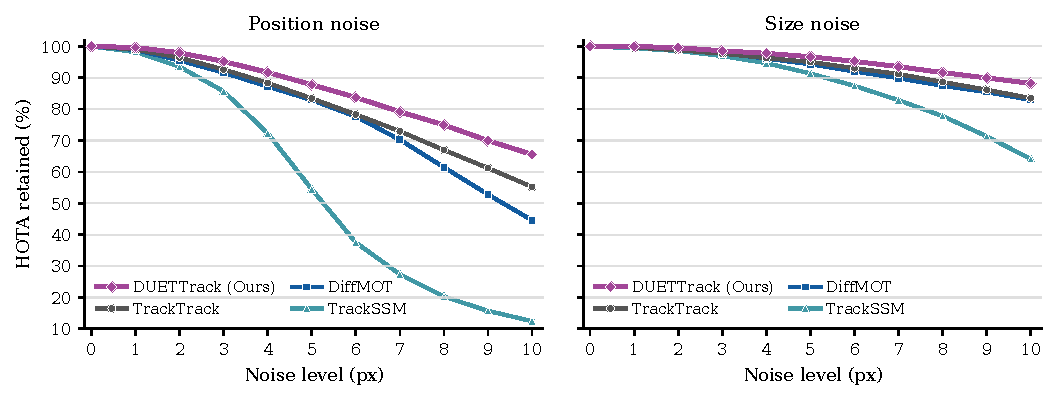
\includegraphics[width=\linewidth]{figures/fig8_duettrack_noise_resistance.pdf}
    \caption{Robustness to increasing position noise (left) and size noise (right) on MOT20 validation. Each curve reports the percentage of HOTA retained relative to that tracker's clean 0-pixel result. Higher is better.}
    \label{fig:noise_robustness}
\end{figure}

Fig.~\ref{fig:noise_robustness} shows that DUETTrack retains the highest fraction of clean HOTA at every nonzero perturbation level. At 10-pixel position noise, DUETTrack retains 65.6\% of its clean HOTA, compared with 55.2\% for TrackTrack, 44.6\% for DiffMOT, and 12.4\% for TrackSSM. Under 10-pixel size noise, the corresponding values are 88.2\%, 83.5\%, 83.0\%, and 64.1\%. The gap over the paired TrackTrack baseline therefore reaches 10.3 retention points for position noise and 4.7 points for size noise at the strongest tested perturbation.

Position perturbations cause a steeper decline than size perturbations for all four trackers, consistent with center displacement directly corrupting apparent motion and the state propagated to the next frame. The controlled TrackTrack comparison is the most direct evidence for DUETTrack: both methods share the surrounding detector, association, and track-management pipeline, while the dual-state assimilation model produces a slower degradation curve. DiffMOT and TrackSSM provide additional cross-method context rather than a component-level causal comparison.

\subsection{Qualitative Analysis}
\begin{figure}[pos=!ht]
    \centering
    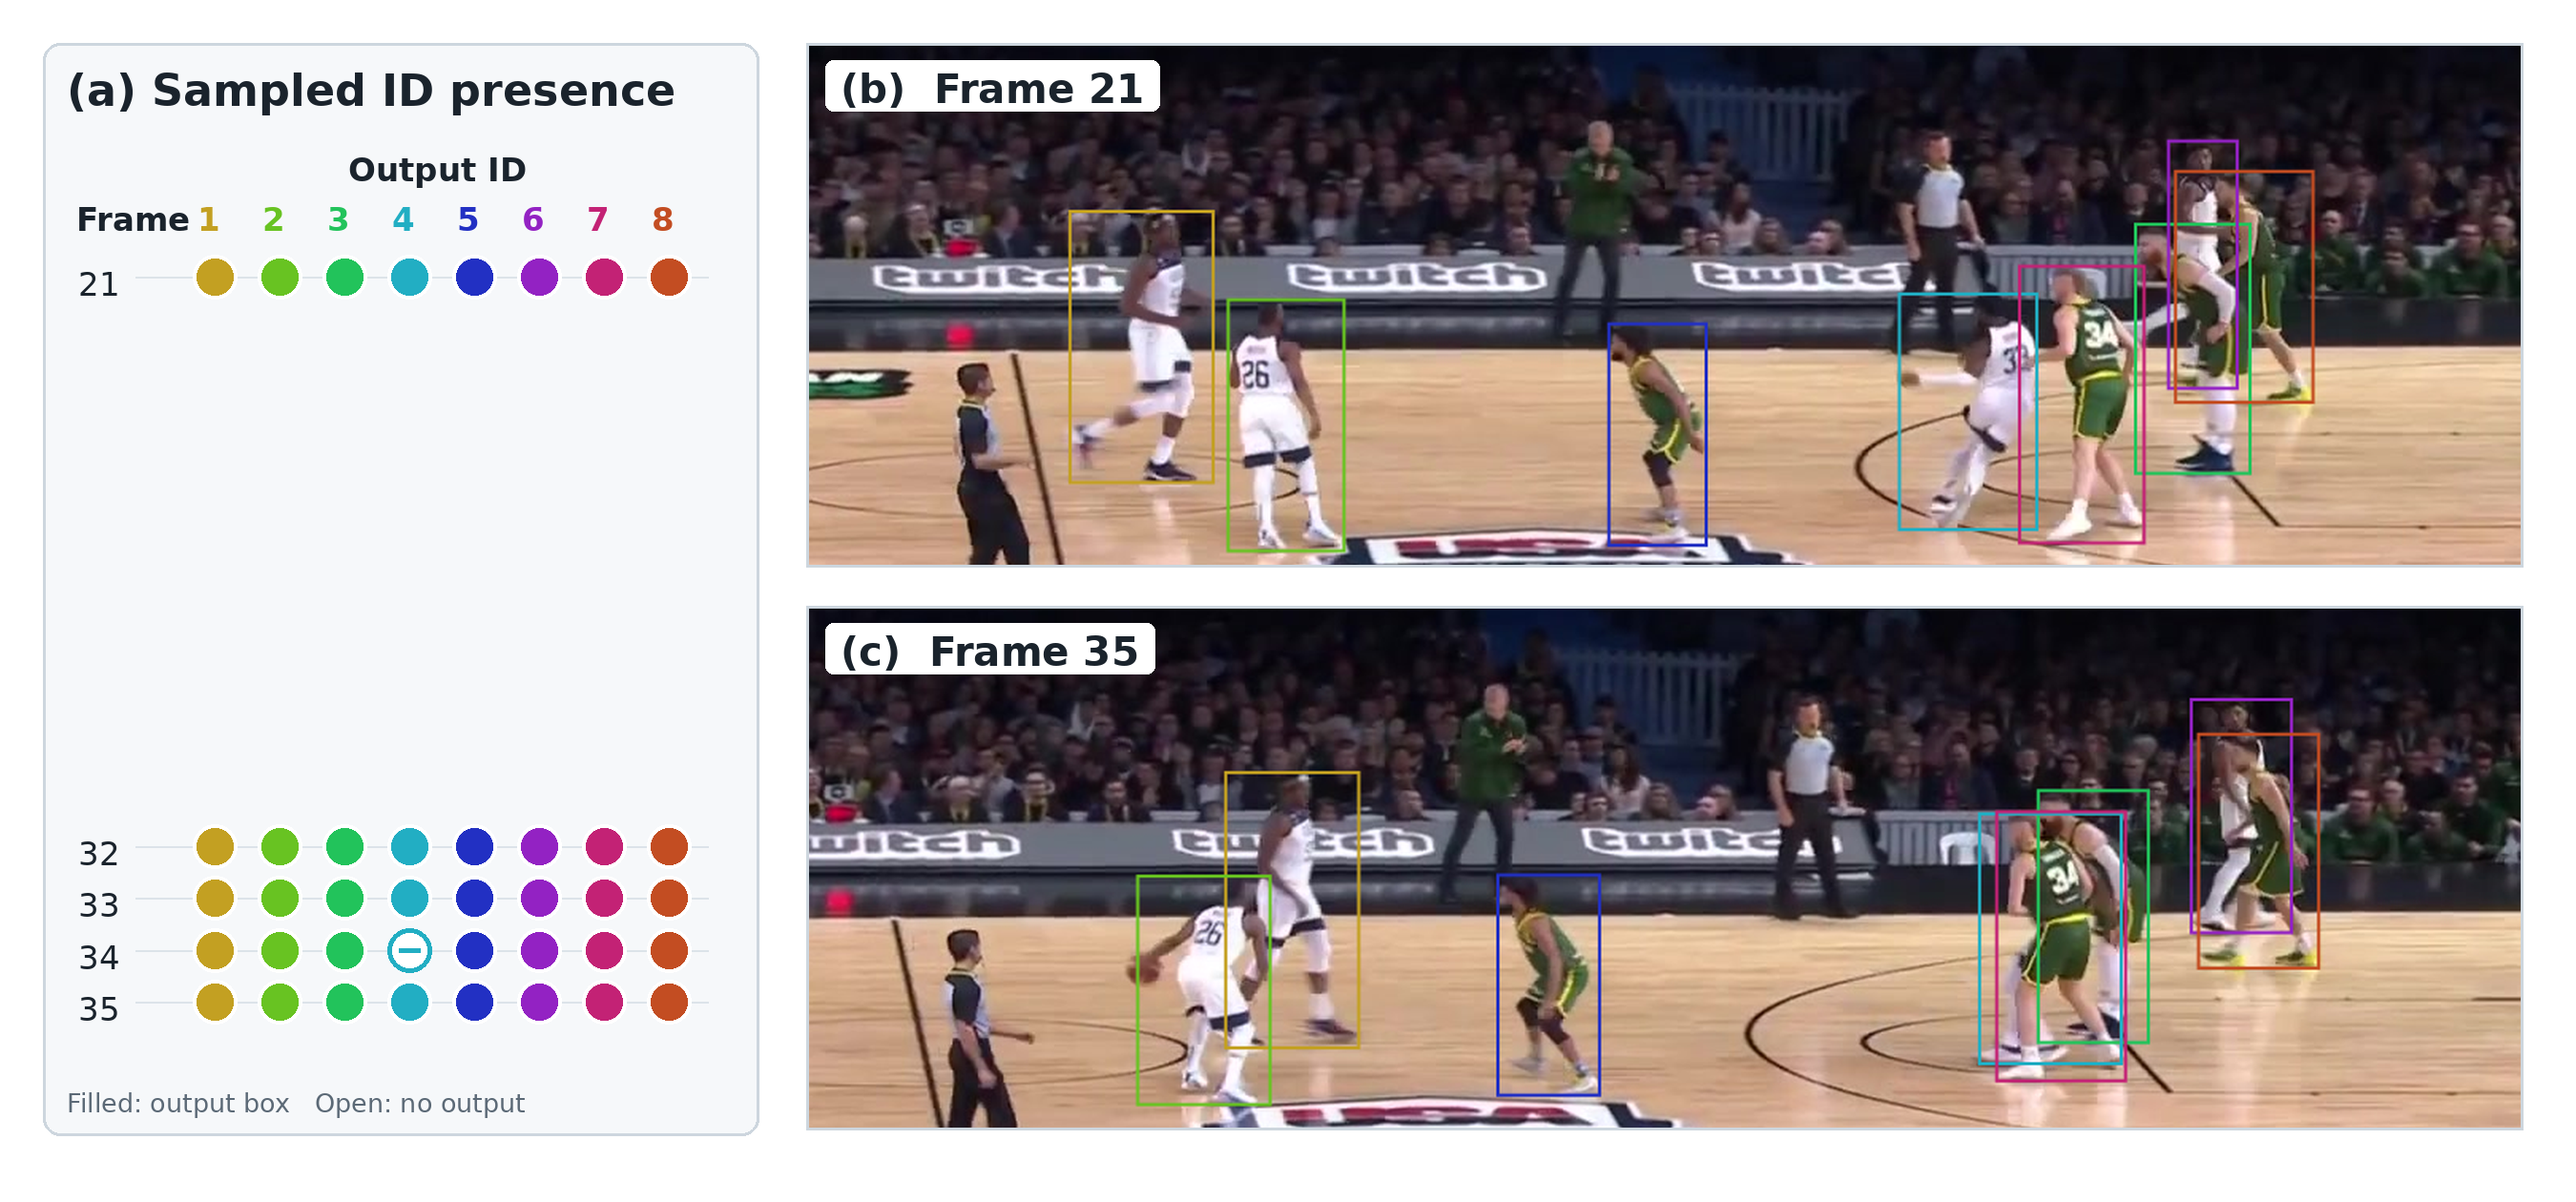
\includegraphics[width=\linewidth]{figures/fig5_sportsmot_scenario_summary.png}
    \caption{Scenario-level output summary on a SportsMOT test clip. Left: sampled presence of output IDs 1--8 at the five supplied frames. A filled marker denotes a rendered box, whereas the open marker records the only absent sampled output, ID 4 at frame 34. Right: full-scene views at frames 21 and 35. The renderer assigns each output ID a deterministic color that is shared across all qualitative panels.}
    \label{fig:qual_scenario}
\end{figure}

\begin{figure}[pos=!ht]
    \centering
    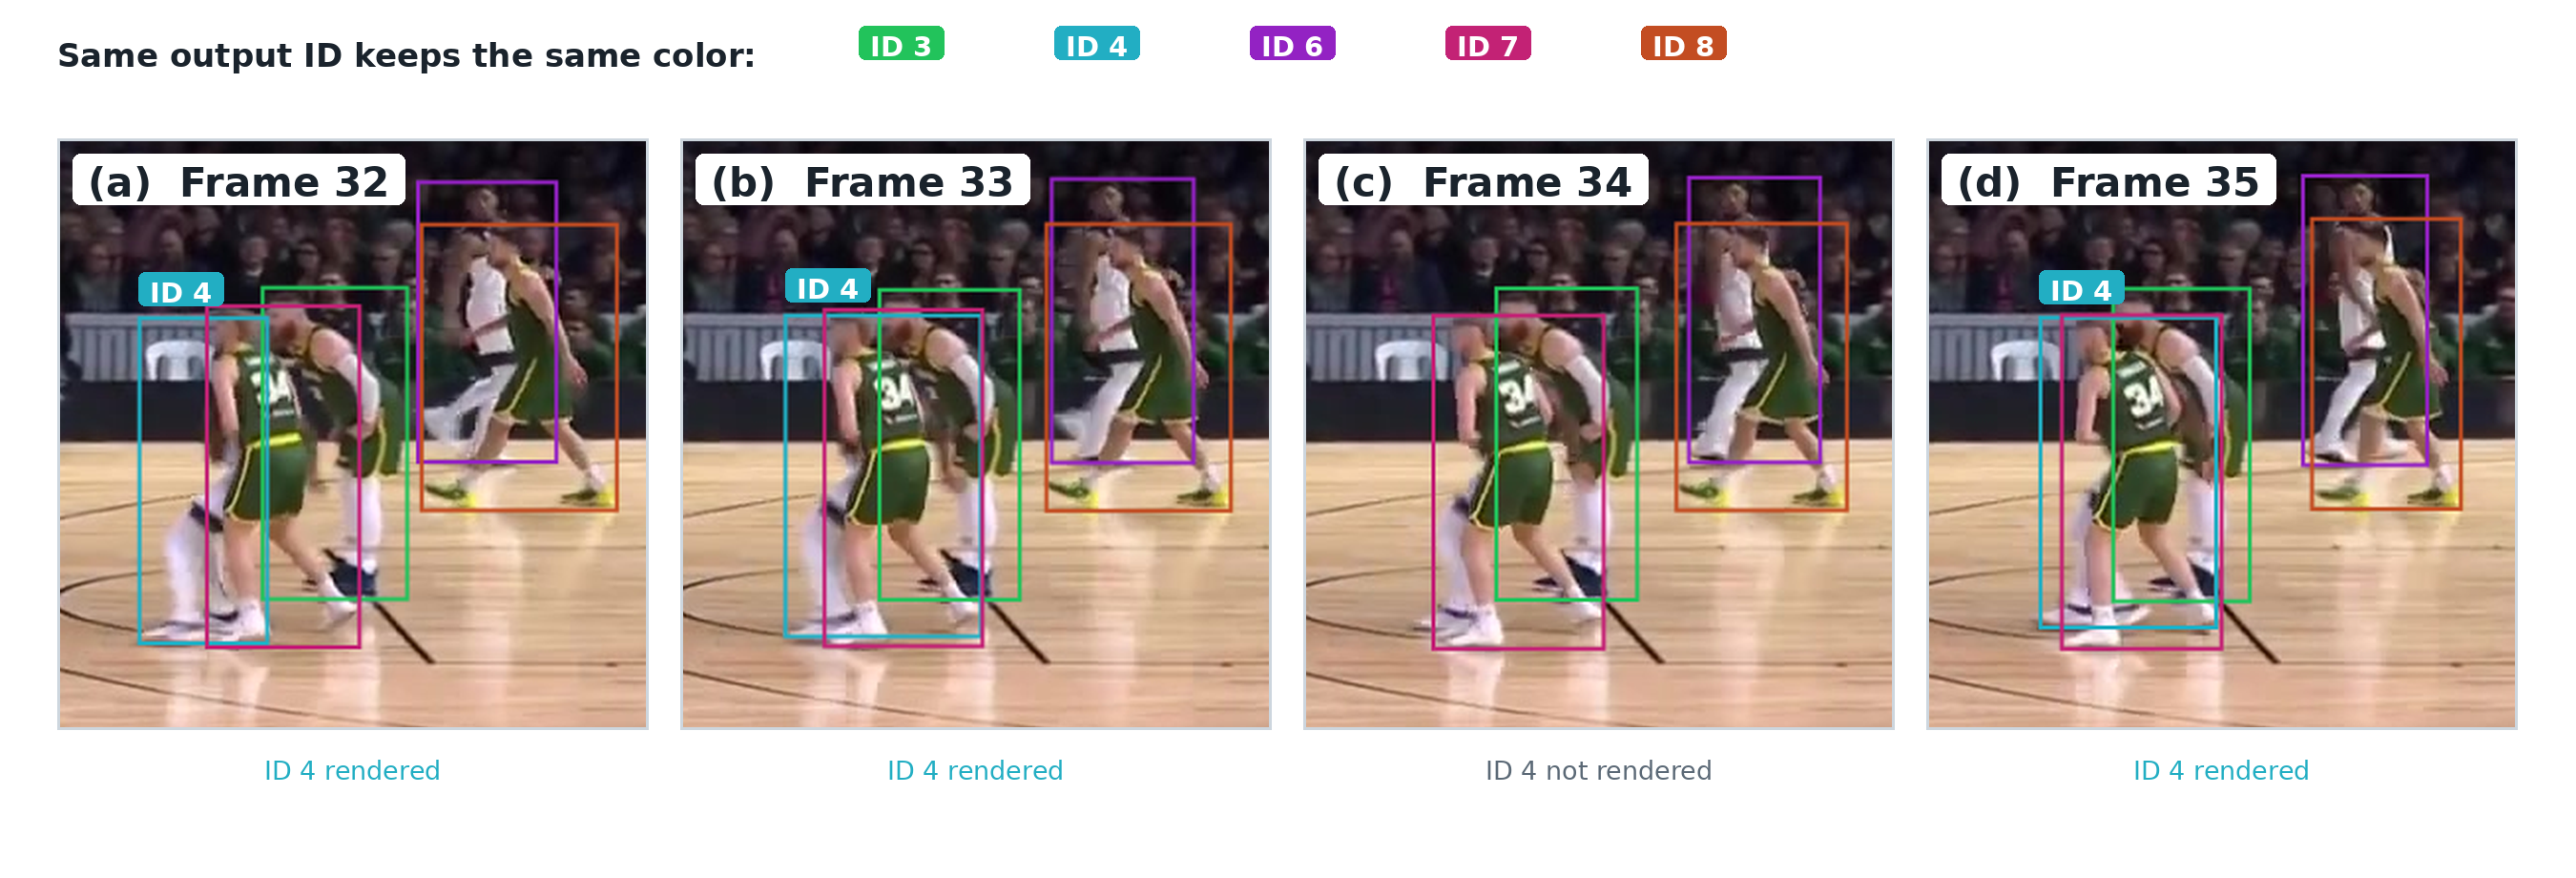
\includegraphics[width=\linewidth]{figures/fig6_sportsmot_crowded_interaction.png}
    \caption{Crowded interaction across four consecutive frames. The fixed crop preserves the same spatial context while five nearby players overlap. ID 4 is rendered at frames 32 and 33, has no output box at frame 34, and is rendered again with the same output identity at frame 35. The remaining colors provide local identity references during the interaction.}
    \label{fig:qual_interaction}
\end{figure}

\begin{figure}[pos=!ht]
    \centering
    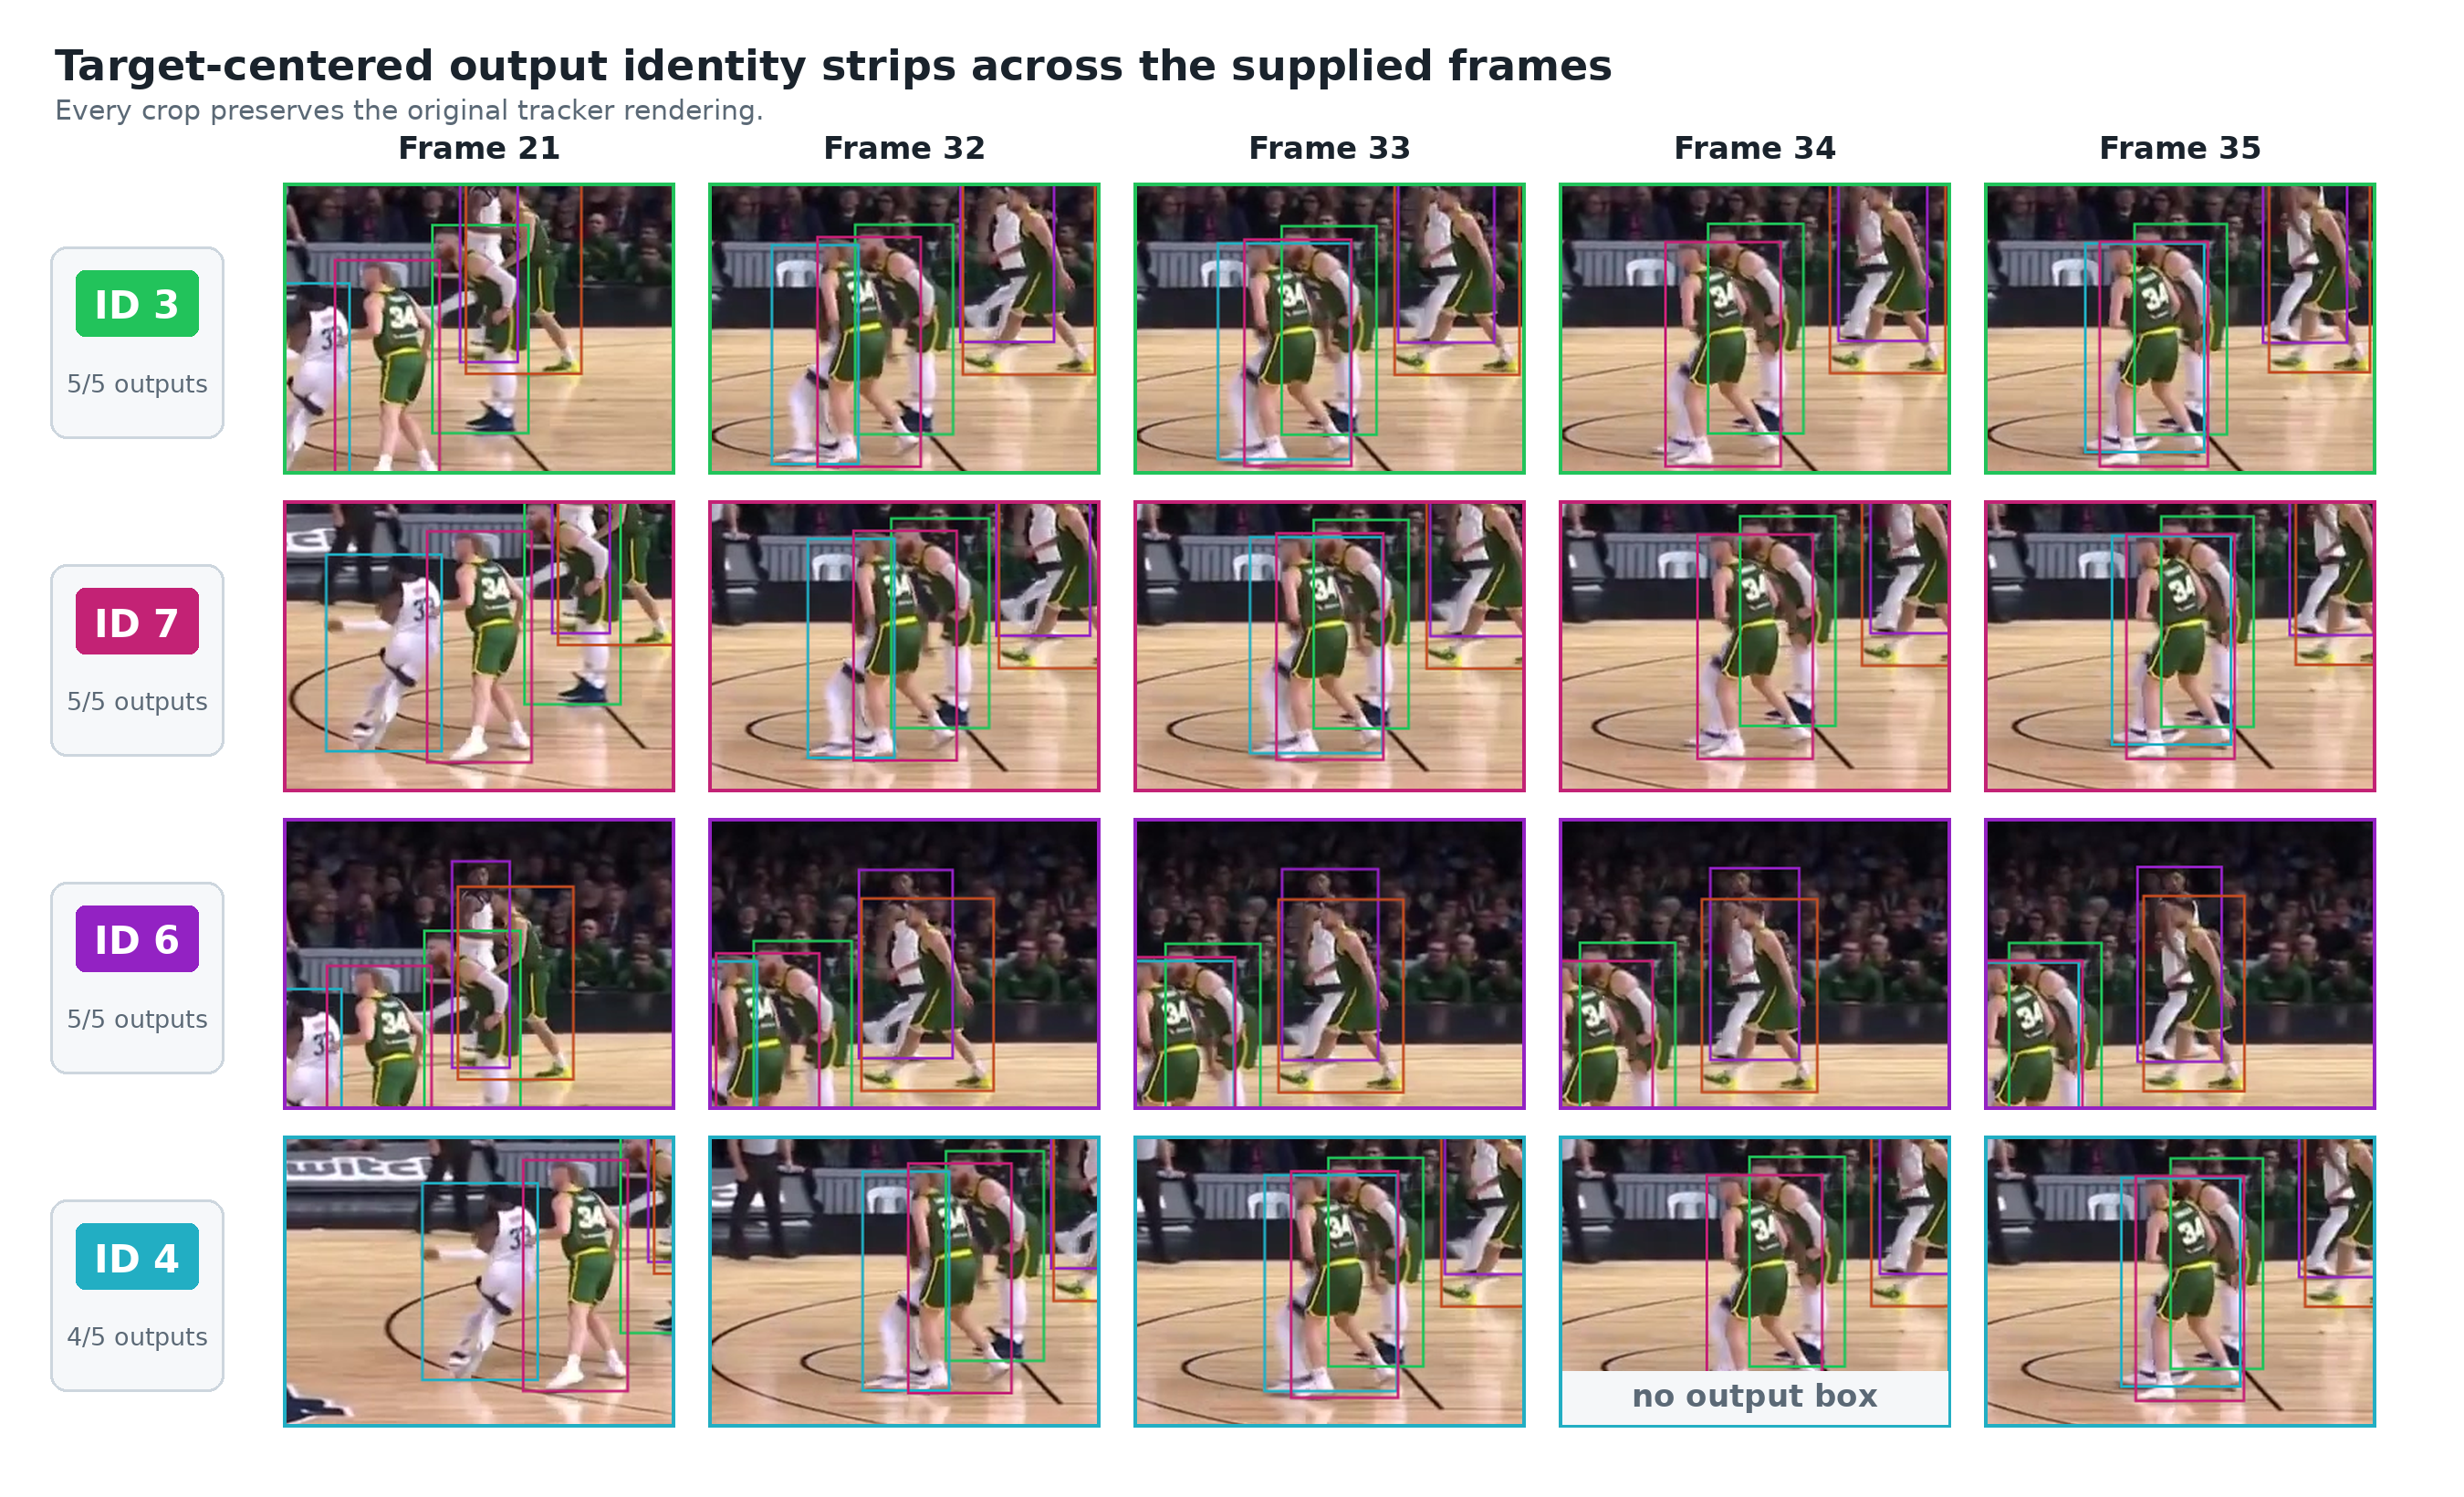
\includegraphics[width=\linewidth]{figures/fig7_sportsmot_identity_strips.png}
    \caption{Target-centered output strips for four representative identities. Each row follows one output ID at the supplied frames 21 and 32--35 using its deterministic color. IDs 3, 7, and 6 are rendered with unchanged identities in all five samples. ID 4 contains one sampled output gap at frame 34 and retains the same output identity when it is rendered at frame 35.}
    \label{fig:qual_strips}
\end{figure}

Fig.~\ref{fig:qual_scenario} adopts the scenario-level organization used in MTUTrack: a temporal identity summary is paired with representative scene frames instead of relying on a full-frame montage alone. All eight output IDs are rendered in frames 21, 32, 33, and 35. The only missing cell among the supplied samples is ID 4 at frame 34. The two scene panels provide the wider basketball context and show that several identities traverse different local neighborhoods between the first and final supplied frames.

Fig.~\ref{fig:qual_interaction} then isolates the most crowded interval with an identical crop at frames 32--35. The cyan ID 4 box is present before the overlap, absent for one supplied frame, and present again at frame 35. Meanwhile, the green ID 3 and magenta ID 7 boxes remain distinguishable inside the central overlap, and the purple ID 6 and orange ID 8 outputs remain stable on the right. Fig.~\ref{fig:qual_strips} reorganizes the same evidence by target rather than by frame, making both uninterrupted sampled identities and the single sampled output gap directly visible.

These output-only examples are consistent with the association-oriented SportsMOT results, including higher AssA and IDF1 and lower IDs and Frag. They do not constitute a ground-truth identity-switch comparison or a causal isolation of CUE and CEC: synchronized TrackTrack renders, test annotations, and coefficient traces are unavailable for this clip. A paired validation figure with identical crops and gate logs is still required to show that a particular baseline error is corrected by motion or appearance assimilation.

\FloatBarrier
\section{Conclusion}
We presented DUETTrack, a post-association framework for utility-guided Kalman-state and appearance-prototype assimilation in online multi-object tracking. Instead of treating every accepted detection as an unconditional write, DUETTrack estimates separate coefficients for the Kalman state and the ReID prototype. CUE learns these coefficients from paired write-versus-hold rollout supervision and a causal history of association, ReID interaction, geometry, Kalman state, and track context. CEC then uses separated state--association and appearance histories with explicit reliability evidence to make bounded coefficient adjustments. Integrated into TrackTrack without changing detection, assignment, or track management, DUETTrack improves HOTA, AssA, and IDF1 on MOT17, MOT20, and SportsMOT while reducing identity switches on all three test sets. The synthetic MOT20 perturbation study further shows that DUETTrack retains a larger fraction of clean HOTA than TrackTrack, DiffMOT, and TrackSSM under both position and size noise. The results indicate that controlling what enters a trajectory after association is a useful complement to improving the association rule itself. Future work will examine occlusion and appearance corruption and relate coefficient trajectories to individual failure modes.

\section*{Acknowledgments}
This work is supported by the National Natural Science Foundation of China (62376106), the Science and Technology Development Plan of Jilin Province (20250102212JC), and the Scientific Research Project of the Jilin Provincial Department of Education (2025KC072).

\printcredits

\bibliographystyle{cas-model2-names}
\bibliography{main}

\end{document}
